% |#########################################################################|
% |                                                                         |
% | Manual for the C++ Reference Manual Indexing Style cc_manual_index.tex  |
% | -------------------------------------------------------------           |
% |                                                                         |
% | 23.09.1999   Susan Hert   hert@mpi-sb.mpg.de                            |
% | Saarbruecken, Germany                                                   |
% | $Revision$                                                        |
% | $Date$                                            |
% |_________________________________________________________________________|
% |#########################################################################|

\documentclass[11pt]{article}
\usepackage{cprog}
\usepackage{cc_manual}
\usepackage{supertabular}
\usepackage{makeidx}
\usepackage{latex_to_html}
\usepackage{epsfig}

\makeindex


% page dimensions
% ---------------
\textwidth 15.4cm
\textheight 24 cm
\topmargin -14mm
\evensidemargin 3mm
\oddsidemargin 3mm

{
  \begingroup
    \catcode`\|=0
    \catcode`\[=1
    \catcode`\]=2
    \catcode`\{=12
    \catcode`\}=12
    \catcode`\\=12
    |gdef|Open[[|tt {]]
    |gdef|Close[[|tt }]]
    |gdef|Backslash[[|tt \]]
  |endgroup
}


\newenvironment{indexex}{\begin{tabbing}
xxxx\=xxx\=\kill}{\end{tabbing}}

\newcommand{\Mindex}[1]{\index{#1@\protect\Backslash{\tt #1}}}
\newcommand{\Eindex}[1]{\index{#1 environment@{\tt #1} environment}}
\newcommand{\ccIndexEntry}[1]{\index{cc#1@\protect\Backslash{\tt cc#1}}}
\newcommand{\TTindex}[1]{\index{#1@{\tt #1}}}
\newcommand{\Dindex}[1]{#1\index{#1}}
\newcommand{\VarText}[1]{$<${\em #1}$>$}

\title{\cgal\ Reference Manual Index Specification \\
         and Style File Documentation}

\author{Susan Hert}

\date{\ccRevision. \ccDate}

\begin{document}

\maketitle


\section{Introduction}
\label{introduction}

This document provides a specification of the format and content of
the index to be produced for the \cgal\ reference manual, and documentation
of tools that may be used to produce such an index.
The specification and tools described in this document
were written with the following goals in mind:
\begin{itemize}
   \item All key words, phrases, topics, and concepts should be indexed.
   \item All \cgal\ \CC\ identifiers described in the manual should be indexed.
   \item There should be listings in the index for any pages on which an 
         item is introduced, defined, or described as well as any pages 
         where key uses for or instances of these things are described.
   \item There should be sufficient cross referencing to allow users
         to find things starting from many different points.
   \item There should NOT be entries for every mention of every item in the
         manual.
\end{itemize}

One \LaTeX\ style file and two Perl scripts have been written to assist in
the  attainment of these goals.  The style file, \verb|cc_manual_index.sty|, 
was written as a companion
to the style file \verb|cc_manual.sty|\TTindex{cc\_manual.sty} and is meant 
to be used in
conjunction with \LaTeX's {\tt makeindex} program.  Minor changes to
\verb|cc_manual.sty| have been made to provide automatic indexing where
possible.  These changes are documented here as well.  The Perl scripts,
{\tt add\_part\_num}\TTindex{add\_part\_num} and {\tt index\_fix}\TTindex{index\_fix}, 
modify the index files generated by
\LaTeX\ and {\tt makeindex}, respectively, to generate an index as specified
in this document.

The general layout of the index is described in Section~\ref{layout}.
There, the specification of how page numbers will appear, which fonts
will be used, how the entries will be ordered, and what vertical and 
horizontal spacing will be used is given. This section also provides
a listing of the categories of things that will be indexed.  
Before delving into a detailed discussion of the contents of the style
file (Section~\ref{style_file}) and how indexing will be done for
each category of items identified in Section~\ref{layout} 
(Section~\ref{how_to_index}), the basic steps necessary for producing
an index that conforms to the layout described in Section~\ref{layout}
is provided in Section~\ref{producing_index}.  

%A sample index produced using these indexing tools has been included
%at the end of the document.  This index was produced from {\tt .tex} files,
%for Chapters 1 through 5 of Part 1 and Chapter 8 of Part 2 of
%the \cgal\ Reference Manual, release 1.1, and
%updated to reflect the introduction of the \cgal\ namespace.

\section{General layout}
\label{layout}

\subsection{Page numbering}%
\label{page_numbering}

There will be a single, global index for all parts of the manual.
To distinguish the pages in each separately numbered part of the manual,
page numbers in the index will be of the form $p.n$, where $p$ is the part 
number and $n$ is the page number in that part\index{part numbers}.  Should 
the manual not
be divided into separately numbered parts, the part number prefixes will 
not be added (Section~\ref{producing_index}).

Items with descriptions spanning several pages will be indexed using page 
ranges ({\it e.g.}, 34--43), since the {\tt makeindex} program can handle 
this quite nicely.
To accomplish this, the beginning and end of the descriptive
text must be marked with indexing commands.  Macros and environments
are provided to do this for all appropriate categories of items.

Multiple page numbers for a single entry will be in numerical order, separated
by commas.   In most cases, {\tt makeindex} will eliminate duplicate page
numbers for a given entry, but it will not do this when, for example,
the same page number is listed in two different fonts.  In such cases,
the program will print a warning in its log file. Such warnings should
be heeded and attempts should be made to remove them so as to avoid
entries such as:
\begin{indexex}
convex hull,   1, {\bf 1}
\end{indexex}%


\subsection{Fonts}%
\index{font|(}
\label{fonts}

There will be three fonts used in the index:
\begin{itemize}
   \item {\verb|\ccFont| } -- \CC\ identifiers will appear in \verb|\ccFont|,
         the same font as in the manual\index{font!ccFont@\verb+\ccFont+}.
   \item {\bf boldface} -- Page numbers on which definitions
         of index entries appear will be in boldface\index{font!boldface}%
         \index{definition}.
   \item {default font} -- All other things will be in default font
         of the rest of the manual\index{font!default}.
\end{itemize}

In the indexing style file, fonts are defined for each of the categories
of items that are not \CC\ names to allow for the easy introduction of other
fonts to distinguish these items in the index should it seem necessary.  
All of these fonts are currently defined to be the default font.
(Actually, they are defined to be empty, but the result is the same.)%
\index{font|)}

\subsection{Ordering of entries}%
\index{ordering of entries|(}%
\label{ordering}

Entries in the index will be in lexicographical order without regard to
case, with the following exception and additions:  
\begin{itemize}
   \item words containing capital letters will come before words with
         only lower case letters when the words
         are otherwise the same
         ({\em e.g.}, the entry for \ccc{\ccFont Orientation} will 
          immediately precede the one for \ccc{\ccFont orientation});
   \item nonalphabetic symbols will be in order by ASCII value, before 
         alphabetic entries;  
   \item non-\CC\ names will come before \CC\ names
         ({\em e.g.}, the entry for the member function \ccc{\ccFont vector} 
          will follow the entry for vector, the general term.)
\end{itemize}
\index{ordering of entries|)}%

\subsection{Spacing}%
\index{spacing|(}
\label{spacing}

The index is formatted in two columns with indexed page numbers 
separated by a comma from the 
text of an entry.  There are three levels of index entries available:
items, subitems, and subsubitems.  Subitems are indented approximately
4 characters from the column in which items begin; subsubitems are indented
approximately 2 characters from the column in which subitems begin. 

There will be one blank line before each main entry that starts with a new 
letter.  There will also be a blank line before each main item that begins
with the \ccc{CGAL_} prefix and a new letter after the prefix.

At times there may be two (or more) options for an entry's presentation, one
that uses fewer lines but more text per line and one that uses shorter
entries but more lines.  For example:
        \begin{indexex}
        conversion  \\
        \> Cartesian to homogeneous,      1.15 \\
        \> homogeneous to Cartesian,      1.15 \\
        \> point to vector,               1.20 \\
        \> vector to point,               1.20 
        \end{indexex}

OR
        \begin{indexex}
        conversion  \\
        \> between number representations, 1.15 \\
        \> between point and vector,       1.20 
        \end{indexex}

Both of these entries will fit in the index without any lines wrapping, but 
since column width is more limited than the number of pages used, when such 
an option presents itself it would be prudent, when in doubt, to opt for 
shorter entries with more lines.%
\index{spacing|)}

\subsection{What to index}
\label{what_to_index}

There are two groups of things that need to be indexed.  The first group
consists of the \CC\ names of all things in \cgal\  that the user has access 
to that are mentioned in the manual.  This group includes the names of:
   \begin{itemize}
      \item assertion flags 
      \item classes
      \item enums
      \item enum tags
%      \item global constants
      \item global functions
      \item global operators
      \item global structs
      \item global variables 
      \item macros
      \item public member functions
      \item typedefs
   \end{itemize}

The second group consists, unfortunately, of things that are not as well 
defined.  These are things other than the \CC\ code
that a user may want or needs to know about in order 
to use the library.  These include:
   \begin{itemize}
      \item abbreviations ({\em e.g.}, CH, DCEL)
      \item concepts ({\em e.g.}, circulator, point, representation class, tree)
      \item functionalities ({\em e.g.}, converting between points and vectors,
                             traversal of a polygon, intersections, distances)
%      \item generic data structures ({\em e.g.}, tree, circle, polygon)
      \item hints about how to do specific things ({\em e.g.}, choosing a 
            representation class)
      \item other libraries ({\em e.g.}, \leda, STL, Geomview)
      \item packages with no associated class name ({\em e.g}, convex hull)
      \item terms ({\em e.g.}, point, polyhedron, halfedge data structure)
   \end{itemize}

Section~\ref{how_to_index} provides more details about how items in each of 
these categories will be indexed.
It is hoped that most things that need to be indexed will fall into exactly 
one of these categories (or, at least, fall most naturally into one category). 
For items that do not fall into these categories, entries should be 
constructed in keeping with the goals described in the introduction.
These exceptional items can be indexed using the generic
indexing macros described in Section~\ref{generic_macros}.  

\section{Producing the index}
\label{producing_index}

The indexing macros in \verb|cc_manual_index.sty| together with the 
{\tt makeindex} program do almost everything that is required for 
producing the index that conforms to the layout described in 
Section~\ref{layout}. For what they are not able to do, two Perl 
scripts have been provided, one of which modifies the {\tt .idx}
that is produced by \LaTeX\, and the other of which modifies the
{\tt .ind} file produced by {\tt makeindex}.    Thus there are
seven steps necessary to produce an indexed (part of the) reference 
manual.

\begin{enumerate}
   \item Add the following lines to the appropriate {\tt .tex} file
         in the appropriate places:  
         \begin{verbatim}
     \usepackage{cc_manual_index} % in the preamble
     \usepackage{makeidx}         % in the preamble
     \makeindex                   % in the preamble
     \printindex                  % where you want the index to appear
         \end{verbatim}
   \item Add calls to the indexing macros in appropriate places
         in the document (Section~\ref{how_to_index}).
   \item Run \LaTeX, as per usual, until everything settles down.  
   \item Add a part number prefix to the page numbers in the generated 
         \verb|.idx| file using the {\tt add\_part\_num}\TTindex{add\_part\_num}\index{part numbers} script.  The proper 
         usage for this script is
         \begin{quote}
            \verb|% add_part_num| $p$ \verb|<filename>.idx|
         \end{quote}
         where $p$ is an integer corresponding to the part number.
         The original \verb|.idx| file is copied to a file with the
         suffix \verb|.idx.nopart|.
   \item Run makeindex
         \begin{quote}
            \verb|% makeindex <filename>|
         \end{quote}
   \item Run the {\tt index\_fix}\TTindex{index\_fix} script on the generated 
         \verb|.ind| file. The proper usage for this script is:
         \begin{quote}
            \verb|% index_fix [-p] <filename>.ind|
         \end{quote}

         The script performs the following six functions: 
         \begin{itemize}
            \item adds a sentence at the beginning of the index explaining the 
                  use of boldface;\index{font!boldface}
            \item strips trailing commas from ``see also'' entries\index{see also entries};
            \item adds blank lines between CGAL-prefixed entries when the
                  letter after the prefix changes\index{spacing};
            \item adds hyphenation clues for names with underscores\index{hyphenation};
            \item puts a space in between the two characters of ``( )'' and
                  ``[ ]'' operators\index{spacing};
            \item if the {\tt -p} option is specified, reformats the integer
                  page numbers in the file into the $p.n$ format by using the
                  first digit of the page number as the value of $p$.
                  If the {\tt -p} option is not used, no reformatting of page 
                  numbers is done\index{part numbers}.
         \end{itemize}
         The original \verb|.ind| file is copied to a file with the suffix
         \verb|.ind.unfixed|.
   \item Run \LaTeX\ one more time to put the index in place in the document.
\end{enumerate}


\section{The file {\tt cc\_manual\_index.sty}}
\label{style_file}

This section provides a discussion of the contents of
the \verb|cc_manual_index.sty| style file and how to use the indexing 
macros provided therein to achieve the best results.
General guidelines for the use of the macros are given
in Section~\ref{general_guidelines}, followed in 
Section~\ref{auto_index} by an outline of the changes that have been made
to \verb|cc_manual.sty| to produce index entries automatically. 
Section~\ref{how_to_stop} documents the commands that may be
used to prevent index entries from being created, either automatically
or otherwise.

In Section~\ref{generic_macros}, the description
of the indexing commands begins with a listing of the 14 general-purpose
commands, which may be used for indexing items in any of
the identified categories as well as items that do not fall into these
categories.  The remaining indexing commands, which are for specific
categories of items, are described in Section~\ref{how_to_index} along 
with the indexing specifications for their respective categories.

\subsection{General guidelines and comments}
\label{general_guidelines}


To achieve the best results, the following things should be
kept in mind when using the indexing macros.
\begin{itemize}
   \item An indexing command should be placed\index{placement of commands}
         immediately after the
         item that is to be indexed, with no spaces or punctuation
         in between.  This will assure that the proper page number is used.
         However, the commands should not, in general, be placed inside the 
         arguments of other commands.
   \item The following types of arguments\index{arguments} are allowed:
         \begin{itemize}
           \item plain text ({\it e.g.}, \verb|\ccIndexMainItem[t]{circulator}|);
           \item plain text with a font%
                 \index{font!in macro arguments}\index{arguments!with fonts} \\
                 ({\it e.g.}, \verb|\ccIndexSubitem[t]{representation class}{\ccFont Cartesian}|);
           \item one of these 3 shortcut commands defined in
                 \verb|cc_manual.sty|: \verb|\stl|\Mindex{stl}, 
                 \verb|\leda|\Mindex{leda}, \verb|\cgal|\Mindex{cgal}
                 ({\it e.g.}, \verb|\ccIndexMainItem[l]{\leda}|);
           \item macros that expand to plain, unformatted text \\
                 ({\it e.g.}, \verb|\ccIndexMainItem[C]{\ccPureClassName}|)
                 \index{arguments!macros as!with plain text}.
         \end{itemize}
   \item The following types of arguments are NOT allowed:
         \begin{itemize}
           \item text enclosed in a \verb|\ccc| or \verb|\ccStyle| command.  
                 If you want this, please use \verb|\ccFont| as the text font 
                 ({\it i.e.}, \verb|\ccIndexSubitem{main}{\ccFont subitem}|).
                 The macros will detect the presence of \verb|\ccFont| 
                 and do the right thing\index{arguments!in \verb+\ccFont+}%
                 \index{arguments!with \verb+\ccc+ or \verb+\ccStyle+}.
           \item macros that expand to formatted text\index{arguments!macros as!with formatted text}.
                 For example, the use of \verb|\ccClassName| instead of 
                 \verb|\ccPureClassName|\index{arguments!class name as} will 
                 cause very nasty things to happen.  

                 Also, if you have defined a command that expands
                 to something like \verb|{\bf text}| (with or without the 
                 braces), this will cause {\tt makeindex} to complain since 
                 the indexing macros cannot pick off the font in order to
                 produce the proper
                 formatting of ``text''. (The shortcut commands such as
                 \verb|\leda|, which are allowed as stand-alone arguments, 
                 are handled as special cases.)
         \end{itemize}
   \item The following type of argument is not recommended:
         \begin{itemize}
           \item text that contains formatting commands in the interior%
                 \index{arguments!with formatting commands} 
                 ({\it i.e.}, something other than a font at the beginning, as,
                 for example, \verb|\ccIndexSubitem{main}{my \leda\ subitem}|). 
                 It is not possible to do all the necessary parsing of these
                 arguments ({\it e.g.}, to pick out a font at the beginning 
                 or to detect a modifier at the end). When such an
                 argument is detected, a warning message will be produced and,
                 if possible, an index entry will be created, but be warned
                 that it may not be correct.
         \end{itemize}
   \item There are two ways to produce a range of pages ({\em e.g.}, 34 -- 45)
         \index{page range} in the index.  For some categories of items, there 
         are environments 
         defined; the first and last pages in the ranges are indexed when
         you enter and leave the environments, respectively.  There are also
         several generic commands of the form \verb|\ccIndexXBegin| and 
         \verb|\ccIndexXEnd|, where {\tt X} is the level of the entry begin 
         produced (Section~\ref{generic_macros}).  These commands must 
         appear in pairs, and the construction of both commands in any such 
         pair must be {\bf exactly} the same 
         except for the ``{\tt Begin}'' or ``{\tt End}'' in the command name.

         There may be multiple page ranges for a single item, but the
         ranges may not overlap\index{page range!multiple}.
   \item Subitems may be created for non-existent main items%
         \index{subitems!for non-existant main items}.
         The {\tt makeindex} program will do the right thing and list a 
         page number for only the subitem and not for the main item 
         (cf. the member function macro below).  The same is true for 
         subsubitems created for non-existent main items and/or subitems%
         \index{subsubitems!for non-existant entries}.
   \item When creating subitems and subsubitems for existing main items
         and subitems\index{subitems!for existing main items}%
         \index{subsubitems!for existing entries}, care 
         must be taken to assure that the texts of the main item and the 
         subitem given as arguments to these commands are {\bf exactly}
         the same, including fonts, as the text used to create 
         the original main item and subitem.  
   \item Where possible, the indexing commands produce the desired cross 
         referencing\index{cross referencing} entries automatically.  See 
         the descriptions of the 
         specific commands to discover precisely when this is done, and
         see Section~\ref{how_to_stop} to find out how to prevent this
         from happening.
\end{itemize}

\subsection{Changes made to {\tt cc\_manual.sty} for automatic indexing}%
\index{automatic indexing|(}
\label{auto_index}

Seventeen commands in \verb|cc_manual.sty|\TTindex{cc\_manual.sty} have been 
modified to produce automatic indexing of \CC\ items.  They are:

\begin{itemize}
   \item \verb|\begin{ccClass}| and \verb|\end{ccClass}|\Eindex{ccClass} 
         (Section~\ref{classes})

   \item \verb|\begin{ccClassTemplate}| and \verb|\end{ccClassTemplate}|%
         \Eindex{ccClassTemplate} (Section~\ref{classes})

   \item \verb|\begin{ccRefClass}| and \verb|\end{ccRefClass}|%
         \Eindex{ccRefClass} (Section~\ref{classes})

   \item \verb|\ccFunction| (Section~\ref{enums_etc})\ccIndexEntry{Function}
        
   \item \verb|\ccMemberFunction| and \verb|\ccMethod|%
         \ccIndexEntry{MemberFunction}\ccIndexEntry{Method}
         (Section~\ref{member_functions}) 

   \item \verb|\begin{ccRefFunction}| and \verb|\end{ccRefFunction}|%
         \Eindex{ccRefFunction} (Section~\ref{member_functions})

   \item \verb|\ccEnum|\ccIndexEntry{Enum} (Section~\ref{enums_etc})

   \item \verb|\begin{ccRefEnum}| and \verb|\end{ccRefEnum}|%
         \Eindex{ccRefEnum} (Section~\ref{enums_etc})


   \item \verb|\ccStruct|\ccIndexEntry{Struct}  (Section~\ref{enums_etc})

   \item \verb|\ccTypedef|\ccIndexEntry{Typedef}  (Section~\ref{enums_etc})

   \item \verb|\ccVariable|\ccIndexEntry{Variable}  (Section~\ref{enums_etc})

   \item \verb|\begin{ccRefVariable}| and \verb|\end{ccRefVariable}|%
         \Eindex{ccRefVariable} (Section~\ref{enums_etc})

   \item \verb|\begin{ccRefMacro}| and \verb|\end{ccRefMacro}|%
         \Eindex{ccRefMacro} (Section~\ref{macros})

   \item \verb|\begin{ccRefConcept}| and \verb|\end{ccRefConcept}|%
         \Eindex{ccRefConcept} (Section~\ref{concepts})

\end{itemize}

For descriptions of precisely what these commands do (and don't
do) with respect to the index, see the sections indicated after
their names.

In addition, three new environments, one for packages and two for
traits classes, have been defined to facilitate automatic indexing.
These environments are:
\begin{itemize}
   \item \verb|\begin{ccPackage}{package}| \ldots
         \verb|\end{ccPackage}|\Eindex{ccPackage} (Section~\ref{packages})
   \item \verb|\begin{ccTraitsClass}{traits_class}{class list}{package list}| 

          \ldots 

         \verb|\end{ccTraitsClass}|\Eindex{ccTraitsClass} (Section~\ref{classes})
   \item \verb|\begin{ccTraitsClassTemplate}{traits_class}{class list}{package list}|

          \ldots

         \verb|\end{ccTraitsClassTemplate}|\Eindex{ccTraitsClassTemplate} (Section~\ref{classes})
\end{itemize}

The package environment\index{packages} requires a single argument, which is 
the name
of the package begin described.  The traits class environments\index{traits classes}
each require three arguments: the first argument supplies the name
of the traits class; the second argument should be a semicolon-separated  
list of classes for which this is a traits class; the third argument
should be a semicolon-separated list of packages for which this is a
traits class.  For example:
\begin{verbatim}
   \begin{ccTraitsClass}{traits_class}{class_1; class_2}{package}
     . . . <description of traits_class> . . .
   \end{ccTraitsClass}
\end{verbatim}
Note that the list of names in the second argument should be simple
class names without template parameters or any other decoration.
Either of the last two arguments for the traits class environments
may be empty.  

But for the index entries produced,
the traits class environments behave exactly 
the same as the {\tt ccClass} and {\tt ccClassTemplate} environments, 
respectively.

In some (hopefully rare) cases, the automatic indexing that is done
by these commands may not be desirable.  The following section describes how 
to turn off the automatic indexing.
\index{automatic indexing|)}
 
\subsection{How to stop indexing}%
\index{preventing indexing|(}
\label{how_to_stop}

Any text that is designated as \verb|\ccHidden|\ccIndexEntry{Hidden} obviously 
produces no index 
entries, but there may be other cases when you wish to prevent commands from
producing index entries.  For example, when the text of a main entry 
contains a comma ({\em e.g.}, {\tt tree, segment}) it is assumed that
the text after the comma is a modifier\index{modifiers} and therefore a 
cross-referencing
entry of the form ``{\tt segment tree,} {\em see} {\tt tree, segment}''
should be generated unless the text after the comma is one of ``2D'',
``3D'', or ``dD'' (Section~\ref{generic_macros}).  If you do not want such 
cross referencing\index{cross referencing} to
be done, then you can turn off this cross referencing using the
command \verb|\ccModifierCrossRefOff|\ccIndexEntry{ModifierCrossRefOff}.  
For example:
\begin{verbatim}
   \ccModifierCrossRefOff
   . . .point\ccIndexMainItem{point, 9D}
   \ccModifierCrossRefOn
\end{verbatim}

Also, as described in Section~\ref{how_to_index}, 
some commands automatically produce two entries in the index, one of which 
can be considered a cross-referencing entry.  To prevent the creation of
this second entry while still allowing automatic cross referencing for 
text that contains modifiers, the command \verb|\ccNonmodifierCrossRefOff|\ccIndexEntry{NonmodifierCrossRefOff}
can be used.  For example:
\begin{verbatim}
   \ccNonmodifierCrossRefOff
    . . . CH\ccIndexAbbreviation{CH}{convex hull}
   \ccNonmodifierCrossRefOn
\end{verbatim}
To turn off both kinds of automatic cross referencing, the command
\verb|\ccCrossRefOff|\ccIndexEntry{CrossRefOff} should be used.

There are five pairs of commands defined in \verb|cc_manual_index.sty| for
the purpose of turning off (and on) various kinds of automatic indexing.  They
are listed here roughly in order by the number of automatic
indexing commands that are affected.
\begin{itemize}
   \item \verb|\ccModifierCrossRefOff|\ccIndexEntry{ModifierCrossRefOff} and 
         \verb|\ccModifierCrossRefOn|\ccIndexEntry{ModifierCrossRefOn}\index{modifiers!no cross referencing}
         -- Commands in text that is between these two commands
         will not produce cross-referencing entries for main items
         that contain commas in their text (which normally indicate
         modifiers following the comma).  
   \item \verb|\ccNonmodifierCrossRefOff|\ccIndexEntry{NonmodifierCrossRefOff} and 
         \verb|\ccNonmodifierCrossRefOn|\ccIndexEntry{NonmodifierCrossRefOn}\index{cross referencing!nonmodifier}
         -- Commands in text that is between these two commands
         will produce cross-referencing entries automatically for only those
         main items that contain commas in their text. 
   \item \verb|\ccCrossRefOff|\ccIndexEntry{CrossRefOff} and 
         \verb|\ccCrossRefOn|\ccIndexEntry{CrossRefOn}\index{cross referencing!turning off}
         -- Commands in text that is between these two commands
         will produce NO cross-referencing entries of any kind
         automatically.  Thus each command produces a single entry
         for the index.  
   \item \verb|\ccAutoIndexingOff|\ccIndexEntry{AutoIndexingOff} and 
         \verb|\ccAutoIndexingOn|\ccIndexEntry{AutoIndexingOn}\index{automatic indexing!turning off}
         -- Commands in text that is between these two commands will
         not generate index entries automatically, but any of the indexing
         macros used explicitly will produce entries (including cross 
         references) as per usual.
   \item \verb|\ccIndexingOff|\ccIndexEntry{IndexingOff} and 
         \verb|\ccIndexingOn|\ccIndexEntry{IndexingOn}
         -- Commands in text that is between these two commands will produce
         NO index entries, automatic or otherwise.
\end{itemize}
The first three pairs of commands should be used sparingly.
% and the last is
%probably useful only for debugging purposes, but is included here for 
%completeness.
\index{preventing indexing|)}

\subsection{General-purpose indexing macros}%
\index{generic macros|(}
\label{generic_macros}

The general-purpose macros listed in this section are to be used for 
creating items, subitems, and subsubitems in the index, as their names imply. 
Each of them takes an optional argument, which should be used to
specify the category of the entry\index{generic macros!optional argument}
\index{categories of entries}.  The valid values for this argument are:
\begin{itemize}
   \item {\tt C[++]} (for any \CC\ name)
   \item {\tt c[oncept]} 
%   \item {\tt d[ata structure]} 
   \item {\tt f[unctionality]} 
   \item {\tt h[int]} 
   \item {\tt l[ibrary]} 
   \item {\tt p[ackage]} 
   \item {\tt t[erm]} 
\end{itemize}
Only the first character of this optional argument is used, so you could
use, for example, ``{\tt laugh}'' or ``{\tt lachen}'' or any other word that 
begins with ``{\tt l}'' to indicate a library.
By default, the argument is blank, which indicates that the
item being indexed is one without an established category.  In this
case, no formatting of any of the text arguments is done by the command,
unless fonts are provided in the text arguments.
When one of the non-default values is supplied for the argument, the
appropriate font\index{font!main item} is used to format the text
of the main item only.  The default font is used for the 
text of subitems\index{font!subitem}
and subsubitems\index{font!subsubitem}.  If some other font is required for 
the subitem or subsubitem
text, the font should be included as part of the argument.  A font may also
be supplied with the main item text\index{font!main item}, in which case this 
font overrides
the font that would be used for the category specified by the optional argument.

When a main item is indexed with text of the form ``{\tt item, modified}''
(or ``{\tt $\backslash$font item, modified}''),
the indexing macros will automatically generate a cross-referencing
entry of the form ``modified item, {\em see} item, modified''\index{modifiers}% 
\index{cross referencing!modifiers}. 
The modifier is assumed to be everything that follows the first comma in
the text. This happens for all main items with text that contains a 
comma\index{commas in main text}, except in the case when the modifier is one 
of ``2D'', ``3D'', or ``dD'', when no cross-referencing entry is 
required\index{modifiers!2D, 3D, or dD}.  If you do not want the 
cross-referencing entry to appear, 
either do not use a comma in the text of the main item or precede
the command by a \verb|\ccModifierCrossRefOff| or \verb|\ccCrossRefOff|
command 
(Section~\ref{how_to_stop}).  This former option is to be preferred.

There are four commands each for items, subitems, and subsubitems.
These commands allow you to create, for each kind of entry, a listing
with a single page number, a range of page numbers, or a boldface page
number (to indicate definitions).  Additionally, there are two commands
for generating ``see also'' entries either as subitems or as subsubitems.
These entries will be listed with no associated page numbers.

\noindent{\bf Main items}%
\index{main items|(}

\begin{itemize}
\item single page number-- {\verb|\ccIndexMainItem[|{\em category\/}\verb|]{item}|}\ccIndexEntry{IndexMainItem}
%     creates a main item labeled with ``item'' (and formatted
%     in the appropriate font if a category argument is supplied) with
%     a single page number.
\item range of pages -- {\verb|\ccIndexMainItemBegin[|{\em category\/}\verb|]{item}|}\ccIndexEntry{IndexMainItemBegin} and \\
     {\verb|\ccIndexMainItemEnd[|{\em category\/}\verb|]{item}|}\ccIndexEntry{IndexMainItemEnd}\index{page range}
%     create a main item labeled with ``item'' (and formatted in the
%     appropriate font if a category argument is supplied) with the range
%     of pages corresponding to the pages on which these two commands occur.
\item boldface page number -- {\verb|\ccIndexMainItemDef[|{\em category\/}\verb|]{item}|}\ccIndexEntry{IndexMainItemDef}\index{definition}
%     creates a main item labeled with ``item'' (and formatted in the 
%     appropriate font if a category argument is supplied) with a single
%     page number if boldface.
\end{itemize}
\index{main items|)}

\noindent{\bf Subitems}
\index{subitems|(}
\begin{itemize}
\item single page number -- {\verb|\ccIndexSubitem[|{\em category\/}\verb|]{item}{subitem}|}\ccIndexEntry{IndexSubitem}
%     creates a subitem labeled ``subitem'' in the default font under the 
%     main item labeled ``item'' (formatted in the appropriate font if a
%     category argument is supplied) with a single page number.
\item range of pages -- {\verb|\ccIndexSubitemBegin[|{\em category\/}\verb|]{item}{subitem}|}\ccIndexEntry{IndexSubitemBegin} and \\
     {\verb|\ccIndexSubitemEnd[|{\em category\/}\verb|]{item}{subitem}|}\ccIndexEntry{IndexSubitemEnd}\index{page range}

%     create a subitem labeled ``subitem'' in the default font under the
%     main item labeled ``item'' (formatted in the appropriate font if a
%     category argument is supplied) with a range of pages corresponding
%     to the pages on which these two commands occur.
\item boldface page number-- {\verb|\ccIndexSubitemDef[|{\em category\/}\verb|]{item}{subitem}|}\ccIndexEntry{IndexSubitemDef}\index{definition}
%     creates a subitem labeled ``subitem'' in the default font under the
%     main item labeled with ``item'' (formatted in the 
%     appropriate font if a category argument is supplied) with a single
%     page number if boldface.
\item see also entry -- {\verb|\ccIndexSubitemSeeAlso[|{\em category\/}\verb|]{item}{subitem}|}\ccIndexEntry{IndexSubitemSeeAlso}\index{see also entries!subitem}
%     creates a subitem labeled ``{\em see also} subitem'' in the default font 
%     under the main item labeled with ``item'' (formatted in the 
%     appropriate font if a category argument is supplied) with no page number
%     following the subitem.
\end{itemize}
\index{subitems|)}

\noindent{\bf Subsubitems}%
\index{subsubitems|(}
\begin{itemize}
\item single page number -- {\verb|\ccIndexSubsubitem[|{\em category\/}\verb|]{item}{subitem}{subsubitem}|}\ccIndexEntry{IndexSubsubitem}
\item range of pages -- {\verb|\ccIndexSubsubitemBegin[|{\em category\/}\verb|]{item}{subitem}{subsubitem}|}\ccIndexEntry{IndexSubsubitemBegin} and \\
     {\verb|\ccIndexSubsubitemEnd[|{\em category\/}\verb|]{item}{subitem}{subsubitem}|}\ccIndexEntry{IndexSubsubitemEnd}\index{page range}
\item boldface page number -- {\verb|\ccIndexSubsubitemDef[|{\em category\/}\verb|]{item}{subitem}{subsubitem}|}\ccIndexEntry{IndexSubsubitemDef}\index{definition}
\item see also entry -- {\verb|\ccIndexSubsubitemSeeAlso[|{\em category\/}\verb|]{item}{subitem}{subsubitem}|}\ccIndexEntry{IndexSubsubitemSeeAlso}\index{see also entries!subsubitem}
\end{itemize}

All entries in the index, except those for abbreviations, can be 
generated using the commands listed above.
However, as detailed in the following section, shortcut commands are 
provided for indexing all \CC\ items and some of the non-\CC\ items, and 
in some cases indexing entries are generated automatically by
the reference manual formatting commands.
\index{subsubitems|)}
\index{generic macros|)}

\section{Specific Indexing Guidelines}
\label{how_to_index}

Outlined below, for each of the categories of entries listed in 
Section~\ref{what_to_index}, is a description of which pages should be 
indexed, what each kind of entry will look like, which cross references will 
appear, the relevant indexing macros, and, where appropriate, the commands
that generate index entries automatically.  This outline should be considered 
to provide only the minimum requirements for each entry;  in some cases there 
may be additional pages or cross references called for.  

\subsection{\cgal\ \CC\ names}
\label{cgal_names}

\subsubsection{Assertion flags}%
\index{assertion flags|(}
\label{assertion_flags}

\begin{description}
   \item[\bf Which pages]
  
         The index should include a listing for any page on which:
      \begin{itemize}
          \item the general use of assertion flags is described;
          \item the specific uses of assertion flags for 
                a package or class are described 
                ({\em i.e.}, the page on which the section labeled 
                 ``Assertions'' begins).
      \end{itemize}

   \item {\bf What will the entry look like}

      There will be a main item labeled ``assertion flags'' in the default
      font.  Associated with
      this will be the page number where the general use of these flags is
      described.  Subitems under this item will correspond to the name of
      packages for which a description of the use of assertion flags is 
      provided in the manual. 

      For example, 

           \begin{indexex}
           assertion flags,                                 0.3       \\
            \> convex hull,                                 2.135     \\
            \> polygon, 2D,                                 2.3   
           \end{indexex}


   \item {\bf Cross references}\index{cross referencing!assertion flags}
      
      \begin{itemize}
         \item The names of the assertion flags mentioned in the 
               manual will have main entries of their own.
         \item Under each package or class name for which the use of
               assertion flags is mentioned in the manual, there will be
               a subitem labeled ``assertion flags''.
      \end{itemize}

      For the example above, the cross references would be:

      \begin{indexex} 
      \ccc{\ccFont CGAL_CH_CHECK_EXPENSIVE},           2.135  \\
       ...                                                       \\
      \ccc{\ccFont CGAL_POLYGON_NO_PRECONDITIONS},     2.3      \\
       ...                                                       \\
      convex hull,                                     2.135    \\
      \> assertion flags,                              2.135     \\
       ...                                                       \\
      \ccc{\ccFont Polygon_2},                     2.3     \\
      \> assertion flags,                               2.3      \\
      \end{indexex}

   \item {\bf Automatic indexing commands}

         None

   \item {\bf Relevant indexing macros}
       \begin{itemize}
          \item{\verb|\ccIndexAssertionFlagsUse|}\ccIndexEntry{IndexAssertionFlagsUse}
               creates a main item labeled ``assertion flags'' in the default 
               font.  This should be used to index the page on which the 
               general use of assertion flags in \cgal\ is explained.

          \item{\verb|\ccIndexAssertionFlagName{FLAG_NAME}|}\ccIndexEntry{IndexAssertionFlagName}
               creates a main item labeled \ccc{\ccFont FLAG_NAME} in 
               \verb|\ccFont|.

         \item{\verb|\ccIndexAssertionFlag[package name]|}\ccIndexEntry{IndexAssertionFlag}
              creates a subitem labeled with the package name in the default 
              font under the main item ``assertion flags'' and  creates a 
              subitem labeled ``assertion flags'' under the current 
              environment's package or class name.  This macro must be used 
              inside a class environment or a {\tt ccPackage} environment. 
              If cross referencing has been turned off using the
              \verb|\ccCrossRefOff| command (Section~\ref{how_to_stop}),
              the entry under
              the main item ``assertion flags'' will not be generated.

              NOTE: When used in a class environment, the package
              name must be supplied as the value of the optional argument 
              ({\em e.g.}, \verb|\ccIndexAssertionFlag[polygon, 2D]|).  This
              argument is ignored when inside a package environment.
       \end{itemize}


\end{description}

\index{assertion flags|)}
\subsubsection{Classes}
\index{classes|(}
\label{classes}

\begin{description}
   \item{\bf Which pages}

         The index should include a listing for any page on which:
       \begin{itemize}
           \item the class description begins;
           \item the class description ends;
           \item an explanation or use of the class is given,
                 if separated from the class description.
       \end{itemize}

   \item{\bf What will the entry look like}

       The class name will be a main item in \verb|\ccFont|, followed by
       the range of pages that the class description spans. 
                 
       Each class's main entry will have as many of the following subitems as
       are appropriate (and perhaps others):
           \begin{itemize}
              \item assertion flags
              \item creation
              \item design
              \item global functions 
                    \begin{itemize}
                       \item names of groups of operations  ({\em e.g.},
                             utilities, convexity checking)
                    \end{itemize}
              \item implementation
              \item member functions 
                    \begin{itemize}
                       \item names of groups of operations ({\em e.g.},
                             for \ccc{\ccFont Polygon_2} traversal,
                             predicates, random access, input, output)
                    \end{itemize}
              \item nested classes
              \item requirements
              \item traits class
                    \begin{itemize}
                       \item default
                       \item requirements
                       \item ``see also'' reference to name of traits class\index{see also entries!traits class}
                    \end{itemize}
             \item types
           \end{itemize}
      The entries for ``global functions'' and ``member functions'' should 
      each be indexed using the range of pages on which the listing of the two 
      corresponding groups of functions are given.

      For example, the entry for \ccc{\ccFont Polygon_2} would 
      look something like this:
      \begin{indexex}
          \ccc{\ccFont{Polygon_2}},       2.3--2.16   \\
          \> assertion flags,                  2.3      \\
          \> creation,                         2.5      \\
          \> global functions,                 2.9--2.10 \\
          \>\> input,                               2.10  \\
          \>\> output,                              2.10  \\
          \> implementation,                   2.11     \\
          \> member functions,                 2.5--2.9 \\
          \>\> predicates,                     2.7      \\
          \>\> random access,                  2.5      \\
          \>\> traversal,                        2.6    \\
          \> traits class,                       2.3  \\
          \>\> default,                          2.16 \\
          \>\> requirements,                     2.14 \\
          \>\> {\em see also} \ccc{\ccFont Polygon_traits_2}  \\
     \end{indexex}


   \item {\bf Cross references}\index{cross referencing!classes}

         \begin{itemize}
              \item The assertion flags entry will be a subitem under the
                    ``assertion flags'' main item.
              \item The names of the member functions  of the class
                    will be main items with the class name as a subitem.
              \item The names of the global functions will be main items
                    without subitems, referring the reader to the page on 
                    which the function specification is given.
              \item The names of the groups of functions will be main items
                    with the class name as a subitem.
              \item The names of the traits classes will be listed as
                    main items, just as for other classes. 
              \item The names of any example classes or default classes
                    will be listed as main items.
         \end{itemize}
         For the sample entry for \ccc{\ccFont Polygon_2},
         an example of each kind of applicable cross reference is shown here: 
            \begin{indexex}
            assertion flags                    \\
            \> \ccc{\ccFont Polygon_2},  2.3 \\
            ...                                \\
            \ccc{\ccFont bbox}                     \\
            \> \ccc{\ccFont Polygon_2},   2.9 \\
            ...                                \\
            input                              \\
            \> \ccc{\ccFont Polygon_2},   2.10 \\
            ...                                \\
            \ccc{\ccFont Polygon_traits_2}, 2.16 \\
            ...                                      \\
            \ccc{\ccFont transform},            2.10 \\
            \end{indexex}

   \item {\bf Automatic indexing commands}\index{automatic indexing}{classes}
         \begin{itemize}
            \item \verb|\begin{ccClass}{class_name}|\Eindex{ccClass} \ldots \verb|\end{ccClass}|; \\
                  \verb|\begin{ccClassTemplate}{class_name}|\Eindex{ccClassTemplate} \ldots 
                  \verb|\end{ccClassTemplate}| \\
                  \verb|\begin{ccRefClass}{class_name}|\Eindex{ccRefClass} \ldots 
                  \verb|\end{ccRefClass}| 

             When you enter a {\tt ccClass}, {\tt ccClassTemplate}, or 
             {\tt ccRefClass} 
             environment an index entry is automatically generated
             to specify the beginning page number for the
             class description.  Similarly, when you leave one of these
             environments, an index entry indicating the end of the page
             range is automatically generated. 

            \item \verb|\begin{ccTraitsClass}{traits_class}{class list}{package list}|\Eindex{ccTraitsClass}\index{traits class!class}\index{traits class!package} \\
\ldots \\
\verb|\end{ccTraitsClass}|; \\
                  \verb|\begin{ccTraitsClassTemplate}{traits_class}{class list}{package list}|\Eindex{ccTraitsClassTemplate} \\
\ldots \\
                  \verb|\end{ccTraitsClassTemplate}| 

             Note that these two environments each have three arguments.
             The first argument is used to supply the name of the traits class.
             The second argument is used to supply the names of the classes
             for which this is a traits class.  The class names should be
             separated by semicolons and should not contain template parameters.
             The third argument is the list of packages for which this class
             is a traits class.  The names in this list should also be separated
             by semicolons.  Either list may be empty.

             When you enter one of these traits class environments, the
             main index entry for the traits class is generated just as for the
             other two class environments.  In addition, a subsubitem labeled
             ``{\em see also} \ccc{traits_class}''\index{see also entries!traits class} is
             created for each class and package for which this is a traits 
             class under the subitem labeled ``traits class'', unless cross
             referencing has been turned off (Section~\ref{how_to_stop})\index{cross referencing!traits classes}. 

             For example,  the following
             commands will result in the creation of a single entry in the
             index -- the main entry for \ccc{traits_class}\ccIndexEntry{NonmodifierCrossRefOff}. 
\begin{verbatim}
         \ccNonmodifierCrossRefOff
         \begin{ccTraitsClass}{traits_class}{}{package}
         \ccNonmodifierCrossRefOn
          . . . <description of traits_class> . . .
         \end{ccTraitsClass}
\end{verbatim}
            (The same effect
             could be achieved by using \verb|\ccCrossRefOff| and
             \verb|\ccCrossRefOn| instead of \verb|\ccNonmodifierCrossRefOff|
             and \verb|\ccNonmodifierCrossRefOn|.)


            \item \verb|\ccMemberFunction|\ccIndexEntry{MemberFunction} and 
                  \verb|\ccMethod|\ccIndexEntry{Method} --
             These macros automatically generate a subitem for the 
             current class under the main item
             labeled with the function name or operator.  This is true
             for all functions and operators except type conversion operators.

             \item \verb|\begin{ccRefFunction}[class::]{function_name}|\Eindex{ccRefFunction} \ldots 
                  \verb|\end{ccRefFunction}| 

             This environment will automatically generate a subitem for the
             {\tt function\_name} under the main item for {\tt class} with the
             page numbers associated with the range of pages on which the 
             \verb|\begin| and \verb|\end| commands appear.  If
             the optional argument, {\tt class}, is not provided, the function
             is assumed to be a global function, and a main entry
             is created for the function name with the associated range of 
             pages. 
        \end{itemize}
         

   \item {\bf Relevant indexing macros}

         The entries for the member functions are produced by the command
         \begin{itemize}
         \item{\verb|\ccIndexMemberFunction{function_name}|}\ccIndexEntry{IndexMemberFunction}
         \end{itemize}
         which creates a main item that is the function name (with no 
         associated page number) with a subitem that is the current class 
         name (with the proper page number).  Both the function name and class
         name are displayed in \verb|\ccFont|.

         Because classes and packages may have similar subitems and subsubitems,
         the macros for indexing classes have been divided into
         two groups: those exclusively for classes and those that may be used 
         for packages or classes.  These macros must be used with class or
         package environments.
         There are also two macros to be used for generating the subsubitems
         for traits classes of a package or class.  These macros do not
         require you to be within any certain environment.

         For any entries that are not handled by the following commands,
         the generic indexing macros (Section~\ref{generic_macros}) should
         be used with ``{\tt C}'' provided as the value of the optional 
         argument.

         \noindent
         {\bf Macros for Classes Only}

         \begin{itemize}
         \item \verb|\begin{ccIndexClass}{class_name}|\Eindex{ccIndexClass} \ldots 
               \verb|\end{ccIndexClass}|

               This environment requires one argument,
               which is the name of the class being indexed.  This environment
               generates an index entry labeled with the class name and with
               a page range corresponding to the pages on which the
               \verb|\begin| and \verb|\end| commands appear.  This should be
               used only when the automatic indexing done by the other class
               environments is not what you want.
         \end{itemize}

         In order to use the following five commands, the variable 
         \verb|\ccIndexClassName|\ccIndexEntry{IndexClassName} must be nonempty.  
         This generally means the commands must be used inside one of the
         environments that define this variable, namely: {\tt ccIndexClass}, 
         {\tt ccClass}, {\tt ccRefClass}, 
         {\tt ccClassTemplate}, {\tt ccTraitsClass}, 
         {\tt ccTraitsClassTemplate}, or {\tt ccRefConcept}\footnote{This is for
         the case when the description of a concept mimics the description of
         a class.}.  You may also define this variable
         yourself before using one of these commands if the commands must
         be used outside one of these environments.
          
         \begin{itemize}
         \item{\verb|\ccIndexClassCreation|}\ccIndexEntry{IndexClassCreation}\index{creation, of class}
              creates a subitem labeled ``creation'' in the default font under
              the current class's main item.
         
         \item{\verb|\ccIndexClassDefault|}\ccIndexEntry{IndexClassDefault}
              creates a subitem labeled ``default'' in the default font under
              the current class's main item.
         
         \item{\verb|\begin{ccIndexMemberFunctions}|}\Eindex{ccIndexMemberFunctions} \ldots
              {\verb|\end{ccIndexMemberFunctions}|}\index{member functions}
              This environment creates a ``member functions'' subitem in the 
              default font under
              the current class's main item with a page range corresponding
              to the pages on which these two commands appear.
         
         \item{\verb|\ccIndexMemberFunctionGroup{group}|}\ccIndexEntry{IndexMemberFunctionGroup}\index{member function group}
              creates a subsubitem under the current class's 
              ``member functions'' subitem labeled with the text ``group'' in 
              the default font.\index{cross referencing!member function group}
              This macro also creates a main item with text ``group'' in the 
              default font (and no associated page number) and subitem
              \verb|\ccPureClassName| in \verb|\ccFont| with the appropriate 
              page number unless cross referencing has been turned off
              (Section~\ref{how_to_stop}).
         
         \item{\verb|\ccIndexNestedClasses|}\ccIndexEntry{IndexNestedClasses}\index{nested classes}
              creates a subitem labeled ``nested classes'' in the default font 
              under the current class's main item.

         \item{\verb|\ccIndexClassTypes|}\ccIndexEntry{IndexClassTypes}\index{types, in classes}
              creates a subitem labeled ``types'' in the default font 
              under the current class's main item.
         
         \end{itemize}
         
         \noindent
         {\bf Macros for Classes or Packages or Concepts}%
         \index{packages|(}
         
         The following five commands and one environment can be used to 
         create subitems and subsubitems under either a package
         or a class 
         main item.  They require that you be in one of the class environments,
         the {\tt ccRefConcept} environment, 
         or a {\tt ccPackage} environment (Section~\ref{packages}).
         (Since there are only two variables -- 
         \verb|\ccIndexClassName|\ccIndexEntry{IndexClassName} and
         \verb|\ccIndexPackageName|\ccIndexEntry{IndexPackageName} -- used to store 
         the names of the current class (or concept) and package being indexed, 
         it is generally not a good idea to nest package or class environments.
         But if you happen to have a package
         environment inside a class environment, the commands will generate 
         entries for the class.  Otherwise, the commands generate entries for 
         the most deeply nested environment.)

         \begin{itemize}
         \item{\verb|\ccIndexAssertionFlag[package name]|}\ccIndexEntry{IndexAssertionFlag}\index{assertion flags}
              creates a subitem labeled with the package name in the default 
              font under the main item ``assertion flags'' and  creates a 
              subitem labeled ``assertion flags'' under the current 
              environment's package or class name.   The former entry is not
              generated if cross referencing has been turned off 
              (Section~\ref{how_to_stop}).\index{cross referencing!assertion flags}

              NOTE: When this command is used in a class environment, the 
              package name must be supplied as the value of the optional 
              argument 
              ({\em e.g.}, \verb|\ccIndexAssertionFlag[polygon, 2D]|).  
              This argument is optional because for packages it is not 
              required (and is ignored), but it is not optional for classes.  
              It must be supplied.
         
         \item{\verb|\ccIndexDesign|}\ccIndexEntry{IndexDesign}\index{design, package or class}
              creates a subitem labeled ``design'' under the current
              package or class name.
         
         \item{\verb|\begin{ccIndexGlobalFunctions}|} \ldots
              {\verb|\end{ccIndexGlobalFunctions}|}%
              \Eindex{ccIndexGlobalFunctions}%
              \index{global functions!package or class}
              create a subitem labeled ``global functions'' under the package or
              class name with a page range corresponding to the pages on which 
              these two commands appear.
         
         \item{\verb|\ccIndexGlobalFunctionGroup{group}|}%
              \ccIndexEntry{IndexGlobalFunctionGroup}%
              \index{global function group, package or class}
              creates a subsubitem under the current package or class name 
              main item and ``global functions'' subitem labeled with the 
              text ``group'' 
              in the default font. This macro also creates a main item with 
              text ``group'' in the default font and a subitem that is the 
              current package or class name, unless cross referencing has
              been turned off (Section~\ref{how_to_stop}).\index{cross referencing!global function group}
         
         \item{\verb|\ccIndexImplementation|}%
              \ccIndexEntry{IndexImplementation}\index{implementation, package or class}
              creates a subitem ``implementation'' displayed in the default font
              under the current package or class name.
         
         \item{\verb|\ccIndexRequirements|}\ccIndexEntry{IndexRequirements}\index{requirements!package or class}
              creates a subitem labeled ``requirements'' in the default font
              under the current package or class name.
         \end{itemize}%
         \index{packages|)}

         \noindent
         {\bf Macros for Traits Classes}%
         \index{traits classes|(}

         The main entry for a traits class should be created just as for any 
         other class by using the appropriate macros listed above. If the
         automatic indexing done upon entering a traits class environment
         is not what you want, the following two commands can be used to
         generate the page range for the trait class's main entry and the
         cross-referencing entries for associated classes and packages
         \begin{itemize}
             \item \verb|\ccIndexTraitsClassBegin{traits_class}{class list}{package list}|\ccIndexEntry{IndexTraitsClassBegin} and \\
                   \verb|\ccIndexTraitsClassEnd|\ccIndexEntry{IndexTraitsClassEnd}

         \end{itemize}
         The argument specifications are the same as for the traits class
         environments (Section~\ref{auto_index}), but the traits class name 
         supplied as the first argument should not contain template parameters.

         In addition, the following two macros should be used to create the 
         appropriate subitems under the relevant package or class item.
         Both commands have an optional first argument that is used to indicate
         whether the traits class is associated with a package or a class and
         must have a value of either ``{\tt p[ackage]}'' or ``{\tt C[++]}''.
         The default value is ``{\tt C}''.

         \begin{itemize}
         
         \item{\verb|\ccIndexTraitsClassDefault[p_or_C]{associated class or package}|}\ccIndexEntry{IndexTraitsClassDefault}\index{default traits class}
              creates an entry labeled ``default'' displayed in the default 
              font under the
              subitem ``traits class'' under the main item labeled with the 
              package or class name associated with this traits class.  
         

         \item{\verb|\ccIndexTraitsClassRequirements[p_or_C]{associated class or package}|}\ccIndexEntry{IndexTraitsClassRequirements}\index{requirements!traits class}
              creates a subsubitem under the package or class name main item and
              ``traits class'' subitem labeled ``requirements'' in the default 
              font.
         \end{itemize}
         \index{traits classes|)}
         
         
         
         \end{description}

\index{classes|)}
\subsubsection{Enums,
            enum tags,
            global structs,
            global variables,
%            global constants,
            global functions,
            typedefs}%
\index{enums|(}%
\index{enum tags|(}%
\index{structs, global|(}%
\index{variables, global|(}%
\index{functions!global|see{global functions}}
\index{global functions|(}%
\index{typedefs|(}%
\label{enums_etc}

\begin{description}
   \item{\bf Which pages}

         The index should include a listing for any page on which:
           \begin{itemize}
                \item the item is introduced and described;
                \item an explanation or use of the item is given, if the 
                      explanation is separated from the introduction.
           \end{itemize}
   \item{\bf What will the entry look like} 

        Each of these items will be indexed in \verb|\ccFont| as a main 
        item with no subitems, followed by the page numbers indicated above.  
        For example:
        \begin{indexex}
        \ccc{\ccFont cartesian_to_homogeneous},                  1.15 \\
        \ccc{\ccFont CLOCKWISE},                                 1.7  \\
        \ccc{\ccFont COLLINEAR},                                 1.7  \\
        \ccc{\ccFont Comparison_result},                         1.8  \\
        \ccc{\ccFont COPLANAR},                                  1.7  \\
        \ccc{\ccFont COUNTERCLOCKWISE},                          1.7
        \end{indexex}

   \item {\bf Cross references} 

         None

   \item {\bf Automatic indexing commands}%

          \begin{itemize}
            \item \verb|\ccEnum|\ccIndexEntry{Enum}%
                  \index{automatic indexing!enums}
                  produces main entries for the enum and the enum tags.

            \item \verb|\begin{ccRefEnum}[class::]{enum_name}|\Eindex{ccRefEnum}
                  \ldots 
                  \verb|\end{ccRefEnum}| 
             This environment will automatically generate a subitem for the
             {\tt enum\_name} under the main item for {\tt class} with the
             page numbers associated with the range of pages on which the 
             ``begin'' and ``end'' commands appear.  If
             the optional argument, {\tt class}, is not provided, the enum
             is assumed to be a global enum, and a main entry
             will be created for the enum with the associated range of pages. 

            \item \verb|\ccFunction|\ccIndexEntry{Function}
                  \index{automatic indexing!global functions}%
                  produces a main entry in the index labeled with the function 
                  name and the appropriate page number for all functions
                  that are not operators.  For the behavior with operators, 
                  see Section~\ref{global_operators}. 

            \item \verb|\ccStruct|\ccIndexEntry{Struct}%
                  \index{automatic indexing!structs}
                  produces a main entry for the name of the struct.

            \item \verb|\ccTypedef|\ccIndexEntry{Typedef}%
                  \index{automatic indexing!typedefs}
                  produces a main entry for the name of the defined type.

            \item \verb|\ccVariable|\ccIndexEntry{Variable}%
                  \index{automatic indexing!variables}
                  produces a main entry for the name of the variable.
          \end{itemize}

   \item {\bf Relevant indexing macros}

         \begin{itemize}
            \item{\verb|\ccIndexEnum{Enum_name}|}\ccIndexEntry{IndexEnum}
            \item{\verb|\ccIndexEnumTag{ENUM_TAG_NAME}|}\ccIndexEntry{IndexEnumTag}
            \item{\verb|\ccIndexGlobalStruct{struct_name}|}\ccIndexEntry{IndexGlobalStruct}
            \item{\verb|\ccIndexGlobalVariable{variable_name}|}\ccIndexEntry{IndexGlobalVariable}
%            \item{\verb|\ccIndexGlobalConstant{CONSTANT_NAME}|}\ccIndexEntry{IndexGlobalConstant}
            \item{\verb|\ccIndexGlobalFunction{Function_name}|}\ccIndexEntry{IndexGlobalFunction}
            \item{\verb|\ccIndexTypedef{Typedef_name}|}\ccIndexEntry{IndexTypedef}
         \end{itemize}

        Each of these commands produces a main entry in the index with the 
        text supplied as the argument displayed in \verb|\ccFont|.  

\end{description}%
\index{enums|)}%
\index{enum tags|)}%
\index{structs, global|)}%
\index{variables, global|)}%
\index{global functions|)}%
\index{typedefs|)}%

\subsubsection{Global operators}%
\index{operators!global|(}
\label{global_operators}

\begin{description}
   \item{\bf Which pages}

         The index should include a listing for any page on which:
           \begin{itemize}
                \item the operator is introduced;
                \item an explanation or use of the operator is given, if the 
                      explanation is separated from the introduction.
           \end{itemize}
   \item{\bf What will the entry look like} 

         Each operator will appear as a main item in \verb|\ccFont| with
         no associated page number.  There will be a subitem for the name
         of the class of (one of the) object(s) on which this operator 
         operates, followed
         by a page number on which the function description is given.

         For example:
          \begin{indexex}
          \ccc{!=} \\
          \> \ccc{Polygon_2}, 2.10 \\
          \ccc{>>} \\
          \> \ccc{Polygon_2}, 2.10
          \end{indexex}

   \item{\bf Cross references} 

         None

   \item{\bf Automatic indexing commands}\index{automatic indexing!global operators}
        \begin{itemize}
            \item \verb|\ccFunction|\ccIndexEntry{Function} 
                  produces, for operators, a main entry in the index labeled 
                  with the operator and a subitem under this labeled with the
                  first templated type name in the parameter list.  If there
                  are no templated parameters, a subitem will be produced for
                  the first type name.
        \end{itemize}

   \item{\bf Relevant indexing macros}
         \begin{itemize}
            \item{\verb|\ccIndexGlobalOperator{operator}{class_name}|}\ccIndexEntry{IndexGlobalOperator}
         \end{itemize}
        This macro produces a subitem labeled with the supplied class 
        name under a main item labeled with the operator symbol; both 
        items are displayed in \verb|\ccFont|.  Care should be taken when
        using this macro for operators that contain one of the characters
        that have special meaning either for the {\tt makeindex} program
        (\verb+@, !, |+) or for \LaTeX\ in general (\verb+&, %, ^, ~+). 
\end{description}
\index{operators!global|)}

\subsubsection{Macros}%
\index{macros|(} 
\label{macros}

\begin{description}
   \item{\bf Which pages}

        The index should include a listing for any page on which
        \begin{itemize}
           \item a macro is described;
           \item an explanation of a use of the macro is
                 given, if the explanation is separated from the introduction 
                 of the macro.
        \end{itemize}
   \item{\bf What will the entry look like}

        Each macro name will be a main entry displayed in \verb|\ccFont|. 
        For example
        \begin{indexex}
        \>\ccc{for_all},                 2.45\\
        \end{indexex}

   \item{\bf Cross references}

        None.

   \item{\bf Automatic indexing commands}\index{automatic indexing!macros}
        \begin{itemize}
         \item \verb|\begin{ccRefMacro}[class::]{macro_name}|\Eindex{ccRefMacro} \ldots 
               \verb|\end{ccRefMacro}| 
             This environment will automatically generate a subitem for the
             {\tt macro\_name} under the main item for {\tt class} with the
             range of pages designated by the pages on which the 
             \verb|\begin| and \verb|\end| commands appear.  If
             the optional argument, {\tt class}, is not provided, the macro
             is assumed to be a global macro, and a main entry
             is created for the macro with the associated range of 
             pages. 
        \end{itemize}

   \item{\bf Relevant indexing macros}
        \begin{itemize}
            \item \verb|\ccIndexMacro{macro_name}|\ccIndexEntry{IndexMacro}
                  creates a main entry with text ``macro\_name'' displayed in
                  \verb|\ccFont| and the associated page number.
        \end{itemize}
\end{description}%
\index{macros|)} 

\subsubsection{Member functions}%
\index{functions!member|see{member functions}}
\index{methods|see{member functions}}
\index{operator member functions|see{member functions}}
\index{member functions|(}
\label{member_functions}

\begin{description}
   \item{\bf Which pages}

         The index should include a listing for any page on which:
        \begin{itemize}
           \item the member function is introduced;
           \item an explanation of a use of the function is
                 given, if the explanation is separated from the introduction 
                 of the function.
        \end{itemize}
   \item{\bf What will the entry look like}

        Each member function will be indexed as a main item in \verb|\ccFont|
        with no associated page number.  There will be a subitem for the name 
        of each class with a member function by that name followed by 
        the page number on which the member function's description is given 
        for that class.  

        For example:
        \begin{indexex}
        \ccc{\ccFont cartesian}  \\
        \> \ccc{\ccFont Point_2},                             1.14 \\
        \> \ccc{\ccFont Vector_2},                            1.18 \\
        \> ...
        \end{indexex}

   \item {\bf Cross references}

          None

   \item {\bf Automatic indexing commands}\index{automatic indexing!member functions}

         \begin{itemize}
            \item \verb|\ccMemberFunction|\ccIndexEntry{MemberFunction} and 
                  \verb|\ccMethod|\ccIndexEntry{Method}
                  produce a main entry in the index labeled with the function 
                  name and with the class name as a subitem.  All functions 
                  and operators are indexed except the type 
                  conversion operators\index{operators!type conversion}.

            \item \verb|\begin{ccRefFunction}[class::]{function_name}|%
                  \Eindex{ccRefFunction} \ldots 
                  \verb|\end{ccRefFunction}| 
             This environment will automatically generate a subitem for the
             {\tt function\_name} under the main item for {\tt class} with the
             page numbers corresponding to the pages on which the 
             \verb|\begin| and \verb|\end| commands appear.  If
             the optional argument, {\tt class}, is not provided, the function
             is assumed to be a global function, and a main entry
             is created for the function name with the associated range of 
             pages. 
         \end{itemize}

          
   \item {\bf Relevant indexing macros}

         \begin{itemize}
            \item{\verb|\ccIndexMemberFunction{function_name}|}\ccIndexEntry{IndexMemberFunction}
                 creates a main item that is the function name (without an 
                 associated page number) with a subitem that is the current
                 class name (with the proper page number).  Both the main 
                 item and subitem are displayed in \verb|\ccFont|.  This
                 macro must be used inside a class environment. 

         \end{itemize}

\end{description}
\index{member functions|)}


\subsection{Things in the \cgal\ Reference Manual without \CC\ names}

There are no automatic indexing commands for items without \CC\ names
other than the cross referencing that occurs for main item text containing
modifiers (Section~\ref{generic_macros}), for abbreviations and the indexing
done for concepts described in a {\tt ccRefConcept} environment, as described 
below.

\subsubsection{Abbreviations}%
\index{abbreviations|(}
\label{abbreviations}

\begin{description}
   \item {\bf Which pages} 
 
         None

   \item {\bf What will the entry look like}

         The abbreviation will be a main item in the default font with a 
         subitem that is ``see Unabbreviated Name''.  For example:
                \begin{indexex}
                CH, {\em see} convex hull           \\
                \end{indexex}
         In this way, the index also serves as a glossary for
         important abbreviations used in the library.

   \item {\bf Cross references}\index{cross referencing!abbreviations}  
  
         \begin{itemize}
            \item The unabbreviated name will be listed as a main item.
         \end{itemize}
        
   \item {\bf Relevant indexing macros}

         \begin{itemize}
           \item{\verb|\ccIndexAbbreviation{ABBR}{unabbreviated text}|}\ccIndexEntry{IndexAbbreviation}
                    creates a main item that is the abbreviation in
                    \verb|\ccIndexAbbreviationFont|
                    followed by a ``{\em see} unabbreviated text'' reference
                    in the default font.  This macro also creates
                    a main item for ``unabbreviated text'' in the default font
                    with the appropriate page number\index{cross referencing!abbreviations}, unless cross
                    referencing has been turned off (Section~\ref{how_to_stop}).
         \end{itemize}
\end{description}%
\index{abbreviations|)}

\subsubsection{Concepts}%
\index{concepts|(} 
\label{concepts}

\begin{description}
   \item{\bf Which pages}

         The index should include a listing for any page on which:
           \begin{itemize}
               \item the concept is introduced and defined;
               \item the concept is employed or explained
                     further, if separated from the introduction.
           \end{itemize}
   \item{\bf What will the entry look like}

        The concept will be a main item in the default font with which the 
        above page numbers
        are listed.  The page number where the concept is defined will be in
        boldface. There should be subitems referring readers to specific
        \cgal\ instances of the concepts or basic functionalities that
        can be achieved for the concept.  

        There may also be subitems for variations on a concept,  as in 
        this example:
        \begin{indexex}
        representation class,                                {\bf 1.3} \\
        \> \ccc{\ccFont Cartesian},                           1.4 \\
        \> choosing,                                               1.5 \\
        \> \ccc{\ccFont Homogeneous},                         1.4 \\
        \end{indexex}

        However,
        to make it easier to stay within the three nesting levels available, 
        distinctions among variations (such as
        2D, 3D, and dD, or range trees, segment trees, multilayer trees, 
        and KD-trees) should usually be done using 
        modifiers\index{modifiers} instead of subitems.  The modifier will be 
        placed after the concept name and separated from it with a comma, as in 
        the following example:
        \begin{indexex}
        point, 2D,                                  {\bf 1.11}, 1.13 \\
        \>  conversion between representations,                  1.15 \\
        \>  conversion to/from vector,                           1.20\\
        \>  {\em see also} \ccc{\ccFont Point_2}                \\
        point, 3D,                                  {\bf 1.57}, 1.59 \\
        \> ...                                                       \\
        \> {\em see also} \ccc{\ccFont Point_3}\\
        point, dD,                                  {\bf 1.??}, 1.?? \\
        \> ...                                                       \\
        \end{indexex}

        In the case when a concept's description mimics that of a class,
        the index entries for the concept should mimic those of a class, and 
        the indexing macros described in Section~\ref{classes} should be used
        to produce this entry.

   \item{\bf Cross references}\index{cross referencing!concepts}

        \begin{itemize}
           \item The basic functionalities will be cross referenced, as 
                 described in Section~\ref{functionalities}.  
           \item Each \CC\ name will be listed as a main item
           \item If modifiers are attached to an item, there should
                 be a cross reference for the term with the modifiers placed
                 before the concept name\index{modifiers}.   An exception is 
                 for the modifiers ``2D'', ``3D'', and ``dD''.  These will 
                 produce no cross references.
           \item Any other subitems that might reasonably serve as starting 
                 points 
                 for a search or might be reached via a different path will
                 be cross referenced either as main items or subitems under
                 other items.
        \end{itemize}

        For example:
        \begin{indexex}
        Cartesian                                                     \\
        \> representation class,                                 1.4   \\
        \ccc{\ccFont Cartesian},                           1.4   \\
        . . .  \\
        conversion  \\
        \> between number representations, 1.15 \\
        \> between point and vector,       1.20 \\
        . . .  \\
        \ccc{\ccFont Homogeneous},                          1.4   \\
        homogeneous                                                   \\
        \> representation class,                                 1.4 \\
        . . .                            \\
        \ccc{\ccFont Point_2},   1.13   \\
        . . .                            \\
        range tree, {\em see} tree, range      
        \end{indexex}

   \item {\bf Automatic indexing commands}\index{automatic indexing!concepts}
         \begin{itemize}
            \item \verb|\begin{ccRefConcept}[class::]{concept}|%
                  \Eindex{ccRefConcept} \ldots 
                  \verb|\end{ccRefConcept}| 
             This environment will automatically generate a subitem for the
             {\tt concept} under the main item for {\tt class} with the
             page numbers associated with the range of pages on which the 
             ``begin'' and ``end'' commands appear.  If
             the optional argument, {\tt class}, is not provided, a main entry
             will be created for the concept with the associated range of 
             pages. 
         \end{itemize}

   \item {\bf Relevant indexing macros}

         The generic indexing macros (Section~\ref{generic_macros}) should be 
         used with ``{\tt c}'' supplied as the value of the optional argument.
\end{description}%
\index{concepts|)} 

\subsubsection{Functionalities}%
\index{functionalities|(} 
\label{functionalities}

\begin{description}
   \item{\bf Which pages} 

         The index should include a listing for any page on which:
           \begin{itemize}
               \item the way to achieve this functionality is described.
           \end{itemize}
   \item{\bf What will the entry look like}

        The main item, listed in the default font, should be the word 
        or phrase that captures the
        essence of the thing to be achieved.  If appropriate, subitems 
        will be used for refinements of this essence. For example:
        \begin{indexex}
        conversion  \\
        \> Cartesian to homogeneous,      1.15 \\
        \> homogeneous to Cartesian,      1.15 \\
        \> point to vector,               1.20 \\
        \> vector to point,               1.20 \\
        \end{indexex}

        In an attempt to limit the number of variations that are produced
        for the terms describing these functionalities, a scan through the
        reference manual (release 1.0) has been made to produce these
        terms\index{functionalities!terms}:
        \begin{itemize}
           \item comparison
           \item conversion
           \item composition
           \item customization
           \item difference
           \item distance computation
           \item drawing
           \item generation
           \item input
           \item insertion
           \item intersection checking
           \item intersection computation
           \item output
           \item removal
           \item searching
           \item transformation
           \item traversal
           \item triangulation
           \item union
           \item verification (validity checking)
        \end{itemize}
        Where appropriate, these are the terms that should be used.  When
        no applicable term is available in this list, the word of phrase
        chosen should, as with the above, be a noun ({\it i.e.}, ``comparison''
        rather than ``compare'' or ``comparing'').


   \item{\bf Cross references}\index{cross referencing!functionalities}
        \begin{itemize}
           \item Any subitems that might reasonably serve as starting points 
                 for a search or might be reached via a different path will
                 be cross referenced either as main items or subitems under
                 other items.
           \item Any subitems that are \CC\ names will also appear as main
                 items.
        \end{itemize}

        For example:
        \begin{indexex}
        point, 2D                                           {\bf 1.11},
                                                                 1.13 \\
        \>  conversion between representations,                  1.15 \\
        \>  conversion to/from vector,                           1.20\\
        \end{indexex}

   \item {\bf Relevant indexing macros}

         The generic indexing macros (Section~\ref{generic_macros}) should 
         be used with ``{\tt f}'' supplied as the value of the optional argument.

\end{description}
\index{functionalities|)} 

%\subsubsection{Generic data structures}%
%\index{data structures|(} 
%\label{generic_ds}
%
%\begin{description}
%   \item{\bf Which pages}
%
%         The index should include a listing for any page on which:
%
%           \begin{itemize}
%               \item the data structure is described or defined.
%           \end{itemize}
%
%   \item{\bf What will the entry look like}
%
%        The generic name or category of the data structure will appear as a 
%        main item in the default font with the associated page number of the 
%        definition (in boldface) 
%        or description.  The subitems of these generic data structure names will
%        refer readers to the specific \cgal\ instances of the data structures
%        with ``see also'' entries corresponding to the class names.
%        There may also be subitems for basic functionalities that can be 
%        achieved for the data structure.
%
%        To make it easier to stay within the three nesting levels available, 
%        distinctions among variations on the basic data structures (such as
%        2D, 3D, and dD, or range trees,
%        segment trees, multilayer trees, and KD-trees) should be done using 
%        modifiers instead of subitems\index{modifiers}.  
%        The modifier will be placed after the 
%        generic data structure name and separated from it with a comma, as in 
%        the following example:
%        \begin{indexex}
%        point, 2D,                                  {\bf 1.11}, 1.13 \\
%        \>  conversion between representations,                  1.15 \\
%        \>  conversion to/from vector,                           1.20\\
%        \>  {\em see also} \ccc{\ccFont Point_2}                \\
%        point, 3D,                                  {\bf 1.57}, 1.59 \\
%        \> ...                                                       \\
%        \> {\em see also} \ccc{\ccFont Point_3}\\
%        point, dD,                                  {\bf 1.??}, 1.?? \\
%        \> ...                                                       \\
%        \end{indexex}
%
%
%   \item{\bf Cross references}\index{cross referencing!concepts}
%
%        \begin{itemize}
%           \item The basic functionalities will be cross referenced, as 
%                 described in Section~\ref{functionalities}.  
%           \item Each class name will be listed as a main item
%           \item If modifiers are attached to an item, there should
%                 be a cross reference for the term with the modifiers placed
%                 before the data structure name.   An exception is for the
%                 modifiers ``2D'', ``3D'', and ``dD''.  These will produce
%                 no cross references.
%        \end{itemize}
%        Examples of these cross references would be:
%        \begin{indexex}
%        range tree, {\em see} tree, range      \\
%        . . .                            \\
%        \ccc{\ccFont Point_2},   1.13   \\
%        . . .                            \\
%        conversion  \\
%        \> between number representations, 1.15 \\
%        \> between point and vector,       1.20 \\
%        \end{indexex}
%   \item {\bf Relevant indexing macros}
% 
%         The generic indexing macros (Section~\ref{generic_macros}) should 
%         be used with ``{\tt d}'' supplied as the value of the optional argument.
%
%\end{description}
%\index{data structures|)} 

\subsubsection{Hints}%
\index{hints|(} 
\label{hints}

\begin{description}
   \item{\bf Which pages}

         The index should include a listing for any page on which:
           \begin{itemize}
               \item a hint is given about how to achieve something.
           \end{itemize}
   \item{\bf What will the entry look like}

        In most  cases, these hints will relate to specific packages, classes,
        concepts, {\em etc.} and will therefore be subitems in the
        default font under the appropriate items.  For example:
        \begin{indexex}
        representation class,                                {\bf 1.3} \\
        \> choosing,                                               1.5  \\
        \end{indexex}

        Any hint that is not related to some other topic should be listed
        as a main item in the default font using the same guidelines as
        for a concept (Section~\ref{concepts}).

   \item{\bf Cross references}\index{cross referencing!concepts}

        These entries will likely not require cross referencing.  But, as 
        before, there should be cross references made for any items that
        could reasonably be the starting point of a search or that might 
        be reached by some other path.

   \item{\bf Relevant indexing macros}

        There are two macros that may be used to create a hint subitem or
        subsubitem under another category of entry.  These are:

        \begin{itemize}
           \item{\verb|\ccIndexHintAsSubitem[|{\em category\/}\verb|]{item}{hint}|}\ccIndexEntry{IndexHintAsSubitem}\index{subitems!hints as}\index{hints!as subitems}
           \item{\verb|\ccIndexHintAsSubsubitem[|{\em category\/}\verb|]{item}{subitem}{hint}|}\ccIndexEntry{IndexHintAsSubsubitem}\index{subsubitems!hints as}\index{hints!as subsubitems}
        \end{itemize}
        As with the generic indexing macros, these commands take an optional
        first argument which indicates the category of the main entry.  The 
        default value of this argument is empty indicating a main entry that 
        does not fall into any of the other categories.  The main item text
        will be displayed in the appropriate font for the category indicated
        by the optional argument value (or the default font, if an argument 
        value is not supplied).

        For hints that are themselves main items, the generic indexing
        macros (Section~\ref{generic_macros}) should be used with 
        ``{\tt h}'' supplied as the value of the optional argument.

\end{description}
\index{hints|)} 

\subsubsection{Libraries}%
\index{libraries|(}
\label{libraries}

\begin{description}
   \item{\bf Which pages}

         The index should include a listing for any page on which:
           \begin{itemize}
               \item the library's relevance to \cgal\ is explained;
               \item a description of how to use the library with \cgal\ is
                     given.
           \end{itemize}
   \item{\bf What will the entry look like}

         The name of the library will be a main item in the default font
         with the above associated page numbers listed after it.  
         Subitems may be warranted to describe different aspects of using the 
         library with \cgal\ or different parts of the library that are relevant.  
         For example:
         \begin{indexex}
         \leda,                                                     1.1  \\
         \>windows,                                                ??.?? \\
         \end{indexex} 
   \item{\bf Cross references}\index{cross referencing!libraries} 

         \begin{itemize}
            \item There should be a ``see also \ccc{\ccFont Library_Name}''\index{see also entries!library}
                  subitem for any item that derives its use or functionality
                  from the library.
         \end{itemize}
         For example:
         \begin{indexex}
         \ccc{\ccFont convex_hull_rat_leda_traits_2},   2.146 \\
         \> see also \leda\ 
         \end{indexex}


   \item {\bf Relevant indexing macros}

         The generic macros (Section~\ref{generic_macros}) should be used 
         with ``{\tt l}'' supplied as the value of the optional argument.

\end{description}%
\index{libraries|)}


\subsubsection{Packages}%
\index{packages|(}%
\label{packages}

\begin{description}
   \item{\bf Which pages}

         The index should include a listing for any page on which:
           \begin{itemize}
              \item the package description begins;
              \item the package description ends;
              \item an explanation or use of the package
                    is described, if separated from the introduction.
           \end{itemize}
   \item{\bf What will the entry look like}

        The package name will be a main item in the default font, followed 
        by the above page numbers.  There will be subitems for the package, 
        as appropriate
        to describe its various features.  When a package
        description closely mimics a class description, its index entry 
        should mimic a class entry (Section~\ref{classes}).  For example,
        the entry for the convex hull package would look something like
        this:
        \begin{indexex}
         convex hull, 2D,                                        2.135--2.148 \\
       \> assertions,                                            2.135  \\
       \> extreme points,                                        2.140  \\
       \> convexity checking,                                    2.142  \\
       \> lower and upper hull,                                  2.138  \\
       \> global functions,                                      2.136--2.142 \\
       \> traits class,                                          2.143  \\
       \>\> default,                                          2.143  \\
       \>\> for \leda\ geometry,                       2.145  \\
       \>\> requirements,                                    2.147  \\
          \>\> {\em see also} \ccc{\ccFont convex_hull_traits_2}\\
          \>\> {\em see also} \ccc{\ccFont convex_hull_constructive_traits_2}\\
          \>\> {\em see also} \ccc{\ccFont convex_hull_rat_leda_traits_2}\\
          \>\> {\em see also} \ccc{\ccFont convex_hull_leda_traits_2}\\
       \> utilities,                                             2.139 \\
        \end{indexex}

   \item{\bf Cross references}\index{cross referencing!packages}

        \begin{itemize}
           \item Any subitems that might reasonably serve as starting points 
                 for a search or might be reached via a different path will
                 be cross referenced either as main items or subitems under
                 other items.
           \item Any subitems that are \CC\ names will also appear as main
                 items.
           \item Cross referencing should mimic class cross referencing
                 when the package description mimics a class description.
        \end{itemize}

   \item{\bf Relevant indexing macros}
        \begin{itemize}
            \item \verb|\begin{\ccPackage}{package name}| \ldots
                  \verb|\end{ccPackage}|\Eindex{ccPackage}

                  This environment, like the class environments, generates
                  an index entry labeled with the package name and the range
                  of pages corresponding to the pages on which the
                  \verb|\begin| and \verb|\end| commands
                  appear.  This environment defines a variable 
                  \verb|\ccIndexPackageName|\ccIndexEntry{IndexPackageName} using 
                  the supplied package name.

                  For package descriptions that mimic class descriptions and 
                  thus require similar indexing, the appropriate macros listed 
                  in Section~\ref{classes} should be used in a {\tt ccPackage}
                  environment.

           \item For creating other entries for packages, especially for 
                 packages that do not mimic classes, the generic macros 
                 (Section~\ref{generic_macros}) should be used 
                 with ``{\tt p}'' supplied as the value of the optional 
                 argument.  When inside a {\tt ccPackage} environment, the 
                 variable \verb|\ccIndexPackageName|\ccIndexEntry{IndexPackageName}
                 should be used (instead of the raw text ``{\tt package name}'')
                 to supply the package name as an argument where necessary.  
                 This will assure that all entries for the package will be
                 formatted similarly.
        \end{itemize}

\end{description}
\index{packages|)} 

\subsubsection{Terms}%
\index{terms|(}
\label{terms}

\begin{description}
   \item{\bf Which pages}

         The index should include a listing for any page on which:
           \begin{itemize}
                \item the term is defined;
                \item the term's relevance in \cgal\ is described,
                      if separated from its definition.
           \end{itemize}
   \item{\bf What will the entry look like}

        The term will be a main item in the index in the default font 
        and the page number on which it is defined will be in boldface.
        For example,
        \begin{indexex}
        ring type               {\bf   1.4}
        \end{indexex}
   \item{\bf Cross references} 

         None 

   \item {\bf Relevant indexing macros}

         The generic macros (Section~\ref{generic_macros}) should be used 
         with ``{\tt t}'' supplied as the value of the optional argument.

\end{description}
\index{terms|)}

%\section{Example}
%\label{example}
%
%On the following pages is a sample index for Chapters 1 through 5 of Part 1
%and Chapter 8 of Part 2 of the \cgal\ Reference Manual, release 1.0.  This 
%corresponds to roughly 34 manual pages, which produced 3 index pages.  This 
%suggests that the complete index, for all 421 manual pages, might be close 
%to 40 pages long.
%
%This example demonstrates all categories of entries for which guidelines are
%given here.  It also demonstrates the problem that is born of
%the \ccc{\ccFont CGAL_really_long_name}s.
%The entry ``see also 
%\ccc{\ccFont CGAL\-_convex\-_hull\-_constructive\-_traits\-_2} 
%under the ``traits class'' subitem of the ``convex hull'' package entry 
%is 35.99242pts too wide as presented.  Without the ``also'' it is still 
%17.04794pts too wide.  With the ``also'' but without the 
%``\ccc{\ccFont CGAL_}'' prefix,  it is 3.20427pts too wide.
%Without either the ``also'' or the ``\ccc{\ccFont CGAL_}''
%prefix, it fits.  So this entry can be made to fit on one line, but it is 
%not clear that that will be true for all entries.  I fear the arrival of the
%half edge data structure.
%
%The \verb|\theindex| environment provided by \LaTeX, which was used with this 
%example, will hyphenate words that extend beyond the column margins (although
%it is, in good \LaTeX\ fashion, somewhat picky about how it does this; witness
%the two entries for 
%\ccc{\ccFont CGAL_\-really_\-really_\-really_\-long_\-convex_\-hull_\-constructive_\-traits_\-2} 
%that come before the entry for \ccc{\ccFont CGAL_\-convex_\-hull_\-constructive_\-traits_\-2}, 
%one of which includes hyphenation clues
%in the middle of ``constructive'' and the other of which does not),  but 
%it has to be told, of course, how to hyphenate the words with underscores in 
%them.  This can either be done manually on an as-needed basis, or a hyphenation
%dictionary for the \cgal\ identifiers could be constructed if one does not 
%already exist. 
%
%This sample index was generated {\em manually}, so there are probably errors 
%in it.  Please ignore these errors unless they hinder your attempt to get an 
%idea of what an index conforming to the specifications outlined in this
%document would look like.  

\small
\printindex

% ----------------------------------------------------------------------
\appendix
\section{Quick Reference Guide}
\newcommand{\Indent}{\hspace*{15pt}}

\normalsize
In this appendix we summarize the various commands defined in
{\tt cc\_manual\_index.sty} and {\tt cc\_manual.sty} that produce
index entries and provide either an example of the result or a
brief explanation of what the command does.  In what follows $p$ is the
page number corresponding to the location of the command, or, in the case
of an environment, it is the page number on which the environment begins.
The page number on which an environment ends is denoted $q$.

\small
\begin{tabular}{|p{7.4cm}|p{7.4cm}|} \hline
&  \\
{\large \bf Command} & {\large \bf Example and/or Result} \\
& \\ \hline \hline
\verb|\ccAutoIndexingOff| 
& Turns off the automatic indexing done with the \verb|\cc*| formatting commands
\ccIndexEntry{AutoIndexingOff}  \\ \hline

\verb|\ccAutoIndexingOn| 
& Turns on the automatic indexing done with the \verb|\cc*| formatting commands
(default)
\ccIndexEntry{AutoIndexingOn}  \\ \hline

\verb|\begin{ccClass}{|\VarText{class\_name}\verb|}|
                            &\verb|\begin{ccClass}{My_class}| \\
\VarText{class description} & ... \\
\verb|\end{ccClass}|         &\verb|\end{ccClass}| \\
& \\
& \ccc{My_class}, $p$ -- $q$ 
\Eindex{ccClass} \\ \hline

\verb|\begin{ccClassTemplate}{|\VarText{class\_name}\verb|}|
                            & \verb|\begin{ccClassTemplate}{Gnu<T>}| \\
\VarText{class description} & ... \\
\verb|\end{ccClassTemplate}| & \verb|\end{ccClassTemplate}| \\
& \\
& \ccc{Gnu<T>}, $p$ -- $q$
\Eindex{ccClassTemplate} \\ \hline

\verb|\ccCrossRefOff| 
& Disables all automatic cross referencing
\ccIndexEntry{CrossRefOff}  \\ \hline

\verb|\ccCrossRefOn| 
& Enables automatic cross referencing (default)
\ccIndexEntry{CrossRefOn}  \\ \hline

\verb|\ccEnum{|\VarText{enum\_decl}\verb|}{|\VarText{comment}\verb|}|
&\verb|\ccEnum{ enum E { E1, E2};}{comment}| \\
& \\
&\ccc{E}, $p$ \\
&\ccc{E1}, $p$ \\
&\ccc{E2}, $p$ 
\ccIndexEntry{Enum} \\ \hline

\verb|\ccFunction{|\VarText{header}\verb|}{|\VarText{comment}\verb|}|
&\verb|\ccFunction{int foo( float d);}{comment}| \\
& \\
&\ccc{foo}, $p$
\ccIndexEntry{Function} \\ \hline

\verb|\ccIndexAbbreviation{|\VarText{ABBR}\verb|}%|
\Indent\verb|{|\VarText{unabbreviated}\verb|}| 
& \verb|\ccIndexAbbreviation{CH}{convex hull}| \\
& CH, {\em see} convex hull
\ccIndexEntry{IndexAbbreviation}  \\ \hline

& \verb|\being{ccClass}{Polygon_2}|\\
\verb|\ccIndexAssertionFlag[|\VarText{package}\verb|]|
& \verb|\ccIndexAssertionFlag[polygon, 2D]| \\
& \\
& assertion flags \\
&\Indent polygon, 2D, $p$ \\
& ...\\
& \ccc{Polygon_2} \\
&\Indent assertion flags, $p$
\ccIndexEntry{IndexAssertionFlag} \\ \hline

\verb|\ccIndexAssertionFlagName{|\VarText{FLAG}\verb|}|
& \verb|\ccIndexAssertionFlagName{%| \\
& \Indent \verb|CGAL_CH_CHECK_EXPENSIVE}| \\
& \\
& \ccc{CGAL_CH_CHECK_EXPENSIVE}, $p$ 
\ccIndexEntry{IndexAssertionFlagName}  \\ \hline

\end{tabular}

\pagebreak
\begin{tabular}{|p{7.4cm}|p{7.4cm}|} \hline
&  \\
{\large \bf Command} & {\large \bf Example and/or Result} \\
& \\ \hline \hline

\verb|\ccIndexAssertionFlagsUse| 
& assertion flags, $p$
\ccIndexEntry{IndexAssertionFlagsUse}  \\ \hline

\verb|\ccIndexClassName| 
& the name of the current class being indexed
\ccIndexEntry{IndexClassName}  \\ \hline

\verb|\begin{ccIndexClass}{|\VarText{class\_name}\verb|}| 
& \verb|\begin{ccIndexClass}{Polygon_2}|\\ 
\VarText{class description} & ... \\
\verb|\end{ccIndexClass}| & \verb|\end{ccIndexClass}| \\
& \\
& \ccc{Polygon_2}, $p$--$q$ 
\Eindex{ccIndexClass}  \\ \hline 

& \verb|\being{ccClass}{Polygon_2}|\\
\verb|\ccIndexClassCreation| 
& \verb|\ccIndexClassCreation| \\
& \\
& \ccc{Polygon_2} \\
& \Indent creation, $p$
\ccIndexEntry{IndexClassCreation}  \\ \hline

& \verb|\being{ccClass}{Polygon_2}|\\
\verb|\ccIndexClassDefault|  
& \verb|\ccIndexClassDefault| \\
& \\
& \ccc{Polygon_2} \\
& \Indent default, $p$
\ccIndexEntry{IndexClassDefault} \\ \hline


& \verb|\being{ccClass}{Polygon_2}|\\
\verb|\ccIndexClassTypes| 
& \verb|\ccIndexClassTypes| \\
& \\
& \ccc{Polygon_2} \\
& \Indent types, $p$
\ccIndexEntry{IndexClassTypes} \\ \hline

& \verb|\being{ccClass}{Polygon_2}|\\
\verb|\ccIndexDesign| 
& \verb|\ccIndexDesign| \\
& \\
& \ccc{Polygon_2} \\
& \Indent design, $p$
\ccIndexEntry{IndexDesign} \\ \hline

\verb|\ccIndexEnum{|\VarText{enum\_name}\verb|}| 
& \verb|\ccIndexEnum{Orientation}|\\
& \\
& \ccc{Orientation}, $p$ 
\ccIndexEntry{IndexEnum} \\ \hline

\verb|\ccIndexEnumTag{|\VarText{ENUM\_TAG}\verb|}| 
& \verb|\ccIndexEnumTag{CLOCKWISE}| \\
& \\
& \ccc{CLOCKWISE}, $p$ 
\ccIndexEntry{IndexEnumTag} \\ \hline

\verb|\ccIndexGlobalFunction{|\VarText{func\_name}\verb|}| 
& \verb|\ccIndexGlobalFunction{ch_jarvis}| \\
& \\
& \ccc{ch_jarvis}, $p$ 
\ccIndexEntry{IndexGlobalFunction}  \\ \hline

& \verb|\begin{ccClass}{Polygon_2}| \\
\verb|\ccIndexGlobalFunctionGroup{|\VarText{group}\verb|}|
& \verb|\ccIndexGlobalFunctionGroup{input}|\\
& \\
& \ccc{Polygon_2} \\
& \Indent global functions \\
& \Indent\Indent input, $p$ 
\ccIndexEntry{IndexGlobalFunctionGroup} \\ \hline

& \verb|\begin{ccClass}{Polygon_2}| \\
\verb|\begin{ccIndexGlobalFunctions}| 
& \verb|\begin{ccIndexGlobalFunctions}| \\
\VarText{global functions}  & ...\\
\verb|\end{ccIndexGlobalFunctions}| 
& \verb|\end{ccIndexGlobalFunctions}|  \\
& \\
& \ccc{Polygon_2}\\ 
& \Indent global functions, $p$--$q$ 
\Eindex{ccIndexGlobalFunctions} \\ \hline
\end{tabular}

\pagebreak
\begin{tabular}{|p{7.4cm}|p{7.4cm}|} \hline
&  \\
{\large \bf Command} & {\large \bf Example and/or Result} \\
& \\ \hline \hline


\verb|\ccIndexGlobalOperator{|\VarText{operator}\verb|}%| & \\
\Indent \verb|{|\VarText{class\_name}\verb|}| 
& \verb|\ccIndexGlobalOperator{<<}{Point_2}| \\
& \\
& \ccc{<<} \\
& \Indent\ccc{Point_2}, $p$ 
\ccIndexEntry{IndexGlobalOperator}  \\ \hline

\verb|\ccIndexGlobalStruct{|\VarText{struct\_name}\verb|}| 
& \verb|\ccIndexGlobalStruct{my_struct}| \\
& \\
& \ccc{my_struct}, $p$  
\ccIndexEntry{IndexGlobalStruct} \\ \hline

\verb|\ccIndexGlobalVariable{|\VarText{var\_name}\verb|}|
& \verb|\ccIndexGlobalVariable{some_var}|  \\
& \\
& \ccc{some_var}, $p$
\ccIndexEntry{IndexGlobalVariable}  \\ \hline

\verb|\ccIndexHintAsSubitem[|\VarText{category}\verb|]%| & \\
\Indent \verb|{|\VarText{item}\verb|}{|\VarText{hint}\verb|}|
& \verb|\ccIndexHintAsSubitem[C]{Polygon_2}%| \\
& \Indent\verb|{partitioning}| \\
& \\
& \ccc{Polygon_2} \\
& \Indent partitioning, $p$
\ccIndexEntry{IndexHintAsSubitem}  \\ \hline

\verb|\ccIndexHintAsSubsubitem[|\VarText{category}\verb|]%| & \\
\Indent\verb|{|\VarText{item}\verb|}{|\VarText{subitem}\verb|}{|\VarText{hint}\verb|}|
& \verb|\ccIndexHintAsSubsubitem%| \\
& \Indent \verb|{\ccFont Point_2}{subitem}{hint}|\\
& \\
& \ccc{Point_2} \\
& \Indent subitem \\
& \Indent\Indent hint, $p$
\ccIndexEntry{IndexHintAsSubsubitem} \\ \hline

&\verb|\begin{ccClass}{Polygon_2}| \\
\verb|\ccIndexImplementation| 
& \verb|\ccIndexImplementation|  \\
& \\
& \ccc{Polygon_2} \\
& \Indent implementation, $p$ \\
\ccIndexEntry{IndexImplementation} & \\ \hline

\verb|\ccIndexingOff| 
& causes all indexing commands defined in {\tt cc\_manual\_index.sty} to have no effect
\ccIndexEntry{IndexingOff} \\ \hline

\verb|\ccIndexingOn| 
& activates the indexing commands (default)
\ccIndexEntry{IndexingOn} \\ \hline


\verb|\ccIndexMacro{|\VarText{macro\_name}\verb|}|
& \verb|\ccIndexMacro{for_all}| \\
& \\
& \ccc{for_all}, $p$ 
\ccIndexEntry{IndexMacro} \\ \hline

\verb|\ccIndexMainItem[|\VarText{category}\verb|]{|\VarText{item}\verb|}|
& \verb|\ccIndexMainItem[p]{new package}| \\
&\\
& new package, $p$ 
\ccIndexEntry{IndexMainItem} \\ \hline

\verb|\ccIndexMainItemBegin[|\VarText{category}\verb|]{|\VarText{item}\verb|}|
& \verb|\ccIndexMainItemBegin{\em item}| \\
& ...\\
& \verb|\ccIndexMainItemEnd{\em item}| \\
& \\
& {\em item}, $p$ -- $q$
\ccIndexEntry{IndexMainItemBegin} \\ \hline

%\verb|\ccIndexMainItemDef[|\VarText{category}\verb|]%| & \\
%\Indent\verb|{|\VarText{item}\verb|}|
\verb|\ccIndexMainItemDef[|\VarText{category}\verb|]{|\VarText{item}\verb|}|
& \verb|\ccIndexMainItemDef{defined item}|  \\
& \\
& defined item, {\bf p}
\ccIndexEntry{IndexMainItemDef} \\ \hline
\end{tabular}

\pagebreak
\begin{tabular}{|p{7.4cm}|p{7.4cm}|} \hline
&  \\
{\large \bf Command} & {\large \bf Example and/or Result} \\
& \\ \hline \hline

%\verb|\ccIndexMainItemEnd[|\VarText{category}\verb|]%| & \\
%\Indent\verb|{|\VarText{item}\verb|}|
\verb|\ccIndexMainItemEnd[|\VarText{category}\verb|]{|\VarText{item}\verb|}|
& see \verb|\ccIndexMainItemBegin|
\ccIndexEntry{IndexMainItemEnd} \\ \hline

& \verb|\begin{ccClass}{Polygon_2}| \\
\verb|\ccIndexMemberFunction{|\VarText{func\_name}\verb|}|
& \verb|\ccIndexMemberFunction{is_simple}|  \\
& \\
& \ccc{is_simple} \\
& \Indent\ccc{Polygon_2} 
\ccIndexEntry{IndexMemberFunction} \\ \hline

& \verb|\begin{ccClass}{Polygon_2}| \\
\verb|\ccIndexMemberFunctionGroup{|\VarText{group}\verb|}|
& \verb|\ccIndexMemberFunctionGroup{modifiers}| \\
& \\
& \ccc{Polygon_2} \\
& \Indent member functions \\
& \Indent\Indent modifiers, $p$
\ccIndexEntry{IndexMemberFunctionGroup}  \\ \hline

& \verb|\begin{ccClass}{Polygon_2}| \\
\verb|\begin{ccIndexMemberFunctions}| & 
\verb|\begin{ccIndexMemberFunctions}| \\ 
\VarText{member functions} & ... \\
\verb|\end{ccIndexMemberFunctions}| &
\verb|\end{ccIndexMemberFunctions}|  \\
& \\
& \ccc{Polygon_2} \\
& \Indent member functions, $p$ -- $q$ 
\Eindex{ccIndexMemberFunctions} \\ \hline 

& \verb|\begin{ccClass}{Polygon_2}| \\
\verb|\ccIndexNestedClasses| 
& \verb|\ccIndexNestedClasses| \\
& \\
& \ccc{Polygon_2} \\
& \Indent nested classes, $p$
\ccIndexEntry{IndexNestedClasses} \\ \hline

\verb|\ccIndexPackageName|
& name of the current package being indexed 
\ccIndexEntry{IndexPackageName} \\ \hline


& \verb|\begin{ccClass}{Polygon_2}| \\
\verb|\ccIndexRequirements| 
& \verb|\ccIndexRequirements| \\
&  \\
& \ccc{Polygon_2} \\
& \Indent requirements, $p$ 
\ccIndexEntry{IndexRequirements} \\ \hline

\verb|\ccIndexSubitem[|\VarText{category}\verb|]{|\VarText{item}\verb|}%| & \\
\Indent\verb|{|\VarText{subitem}\verb|}|
& \verb|\ccIndexSubitem{\bf item}{\em subitem}| \\
& \\
& {\bf item} \\
& \Indent {\em subitem}, $p$
\ccIndexEntry{IndexSubitem} \\ \hline

\verb|\ccIndexSubitemBegin[|\VarText{category}\verb|]%| & \\
\Indent\verb|{|\VarText{item}\verb|}{|\VarText{subitem}\verb|}|
& \verb|\ccIndexSubitemBegin[t]{term}{subitem}| \\
& ... \\
& \verb|\ccIndexSubitemEnd[t]{term}{subitem}| \\
& \\
& term \\
& \Indent subitem, $p$ -- $q$
\ccIndexEntry{IndexSubitemBegin} \\ \hline

\verb|\ccIndexSubitemDef[|\VarText{category}\verb|]%| & \\
\Indent\verb|{|\VarText{item}\verb|}{|\VarText{defined subitem}\verb|}|
& \verb|\ccIndexSubitemDef{item}{subitem}| \\
& \\
& item \\
& \Indent subitem, {\bf p}
\ccIndexEntry{IndexSubitemDef} \\ \hline

\verb|\ccIndexSubitemEnd[|\VarText{category}\verb|]%| & \\
\Indent\verb|{|\VarText{item}\verb|}{|\VarText{subitem}\verb|}|
& see \verb|\ccIndexSubitemBegin|
\ccIndexEntry{IndexSubitemEnd}  \\ \hline
\end{tabular}

\pagebreak
\begin{tabular}{|p{7.4cm}|p{7.4cm}|} \hline
&  \\
{\large \bf Command} & {\large \bf Example and/or Result} \\
& \\ \hline \hline

\verb|\ccIndexSubitemSeeAlso[|\VarText{category}\verb|]%| & \\
\Indent\verb|{|\VarText{item}\verb|}{|\VarText{subitem}\verb|}|
& \verb|\ccIndexSubitemSeeAlso[c]{concept}%| \\
& \Indent\verb|{cross-ref}| \\
& \\
& concept \\
& \Indent {\em see also} cross-ref
\ccIndexEntry{IndexSubitemSeeAlso} \\ \hline

\verb|\ccIndexSubsubitem[|\VarText{category}\verb|]%| & \\
\Indent\verb|{|\VarText{item}\verb|}{|\VarText{subitem}\verb|}{|\VarText{subsubitem}\verb|}|
& \verb|\ccIndexSubsubitem{item}{subitem}%| \\
& \Indent\verb|{subsubitem}| \\
& \\
& item \\
& \Indent subitem \\
& \Indent\Indent subsubitem, $p$
\ccIndexEntry{IndexSubsubitem}  \\ \hline

\verb|\ccIndexSubsubitemBegin[|\VarText{category}\verb|]%| & \\
\Indent\verb|{|\VarText{item}\verb|}{|\VarText{subitem}\verb|}{|\VarText{subsubitem}\verb|}|
& \verb|\ccIndexSubsubitemBegin[C]{ident}%| \\
& \Indent\verb|{subitem}{subsubitem}| \\
& ... \\
& \verb|\ccIndexSubsubitemEnd[C]{ident}%| \\
& \Indent\verb|{subitem}{subsubitem}| \\
& \\
& \ccc{ident} \\
& \Indent subitem \\
& \Indent\Indent subsubitem, $p$
\ccIndexEntry{IndexSubsubitemBegin} \\ \hline

\verb|\ccIndexSubsubitemDef[|\VarText{category}\verb|]%| & \\
\Indent\verb|{|\VarText{item}\verb|}{|\VarText{subitem}\verb|}{|\VarText{subsubitem}\verb|}|
& \verb|\ccIndexSubsubitemDef[t]{term}%| \\
& \Indent\verb|{subitem}{defined subsubitem}| \\
& \\
& term \\
& \Indent subitem \\
& \Indent\Indent defined subsubitem, {\bf p}
\ccIndexEntry{IndexSubsubitemDef} \\ \hline

\verb|\ccIndexSubsubitemEnd[|\VarText{category}\verb|]%| & \\
\Indent\verb|{|\VarText{item}\verb|}{|\VarText{subitem}\verb|}{|\VarText{subsubitem}\verb|}|
& see \verb|\ccIndexSubsubitemBegin|
\ccIndexEntry{IndexSubsubitemEnd} \\ \hline

\verb|\ccIndexSubsubitemSeeAlso[|\VarText{category}\verb|]%| & \\
\Indent\verb|{|\VarText{item}\verb|}{|\VarText{subitem}\verb|}{|\VarText{subsubitem}\verb|}|
& \verb|\ccIndexSubsubitemSeeAlso{item}%| \\
& \Indent\verb|{subitem}{cross-ref}| \\
& \\
& item \\
& \Indent subitem \\
& \Indent\Indent {\em see also} cross-ref
\ccIndexEntry{IndexSubsubitemSeeAlso} \\ \hline

\verb|\ccIndexTraitsClassBegin{|\VarText{class}\verb|}%| & \\
\Indent\verb|{|\VarText{class list}\verb|}{|\VarText{package list}\verb|}| 
& \verb|\ccIndexTraitsClassBegin{K_Traits}%| \\
& \Indent\verb|{class1; class2}| \\
& ...\\
& \verb|\ccIndexTraitsClassEnd{K_Traits}%|\\
& \Indent\verb|{class1; class2}| \\
& \\
& \ccc{class1} \\
& \Indent traits class \\
& \Indent\Indent {\em see also} \ccc{K_Traits} \\
& \ccc{class2} \\
& \Indent traits class \\
& \Indent\Indent {\em see also} \ccc{K_Traits} \\
& ... \\
& \ccc{K_Traits}, $p$ -- $q$
\ccIndexEntry{IndexTraitsClassBegin} \\ \hline
\end{tabular}

\pagebreak
\begin{tabular}{|p{7.4cm}|p{7.4cm}|} \hline
&  \\
{\large \bf Command} & {\large \bf Example and/or Result} \\
& \\ \hline \hline


\verb|\ccIndexTraitsClassDefault[|\VarText{p\_or\_C}\verb|]%| & \\
\Indent \verb|{|\VarText{class or package}\verb|}| 
& \verb|\ccIndexTraitsClassDefault[p]%| \\
& \Indent\verb|{convex hull}| \\
& \\
& convex hull \\
& \Indent traits class \\
& \Indent\Indent default, $p$
\ccIndexEntry{IndexTraitsClassDefault} \\ \hline

\verb|\ccIndexTraitsClassEnd{|\VarText{class}\verb|}%| & \\
\Indent\verb|{|\VarText{class list}\verb|}{|\VarText{package list}\verb|}| 
& see \verb|\ccIndexTraitsClassBegin|
\ccIndexEntry{IndexTraitsClassEnd} \\ \hline

\verb|\ccIndexTraitsClassRequirements%| & \\
\Indent\verb|[|\VarText{p\_or\_C}\verb|]{|\VarText{class or package}\verb|}| 
& \verb|\ccIndexTraitsClassRequirements[p]%| \\
& \Indent\verb|{convex hull}| \\
& \\
& convex hull \\
& \Indent traits class \\
& \Indent\Indent requirements, $p$
\ccIndexEntry{IndexTraitsClassRequirements} \\ \hline

\verb|\ccIndexTypedef{|\VarText{type\_name}\verb|}|
& \verb|\ccIndexTypedef{Sleep}| \\
& \\
& \ccc{Sleep}, $p$ 
\ccIndexEntry{IndexTypedef} \\ \hline

&\verb+\begin{ccClassTemplate}{Gnu<T>}+ \\
\verb|\ccMemberFunction{|\VarText{declaration}\verb|}%|
&\verb+\ccMemberFunction{ int f(X x);}{comment}+ \\
\Indent\Indent\verb|{|\VarText{comment}\verb|}| & \\
& \\
& \ccc{gnat} \\ 
& \Indent \ccc{Gnu<T>}, $p$
\ccIndexEntry{MemberFunction} \\ \hline

\verb|\ccMethod{|\VarText{declaration}\verb|}{|\VarText{comment}\verb|}|
& see \verb|\ccMemberFunction|
\ccIndexEntry{Method}\\ \hline

\verb|\ccModifierCrossRefOff|
& turns off automatic cross referencing of words that come after a comma in
the main text of an indexing command
\ccIndexEntry{ModifierCrossRefOff} \\ \hline

\verb|\ccModifierCrossRefOn| 
& turns on automatic cross referencing of words that come after a comma in
the main text of an indexing command (default)
\ccIndexEntry{ModifierCrossRefOn} \\ \hline

\verb|\ccNonmodifierCrossRefOff| 
& turns off all automatic cross referencing except for words that come after 
a comma in the main text of an indexing command
\ccIndexEntry{NonmodifierCrossRefOff} \\ \hline

\verb|\ccNonmodifierCrossRefOn| 
& turns on automatic cross referencing done by some of the commands (default)
\ccIndexEntry{NonmodifierCrossRefOn} \\ \hline

\verb|\begin{ccPackage}{|\VarText{package name}\verb|}|
                              & \verb|\begin{ccPackage}{convex hull}|\\
\VarText{package description} & ... \\
\verb|\end{ccPackage}|        & \verb|\end{ccPackage}| \\
& \\
& convex hull, $p$ -- $q$
\Eindex{ccPackage} \\ \hline

\verb|\begin{ccRefClass}[|\VarText{scope}\verb|]{|\VarText{class\_name}\verb|}|
                             &\verb+\begin{ccRefClass}{A_class<C>}+  \\
\VarText{class description}  & ... \\
\verb|\end{ccRefClass}|      & \verb|\end{ccRefClass}|\\
& \\
& \ccc{A_class<C>}, $p$ -- $q$
\Eindex{ccRefClass} \\ \hline

\verb|\begin{ccRefConcept}[|\VarText{scope}\verb|]%|
& \verb+\begin{ccRefConcept}{Circulator}+ \\
\Indent\Indent \verb|{|\VarText{concept name}\verb|}|  & \\
           \VarText{concept description} & ...\\
\verb|\end{ccRefConcept}|                &  \verb|\end{ccRefConcept}| \\
& \\
& Circulator, $p$ -- $q$
\Eindex{ccRefConcept}\\ \hline
\end{tabular}

\pagebreak
\begin{tabular}{|p{7.4cm}|p{7.4cm}|} \hline
&  \\
{\large \bf Command} & {\large \bf Example and/or Result} \\
& \\ \hline \hline

\verb|\begin{ccRefEnum}[|\VarText{scope}\verb|]|\verb|{|\VarText{enum\_name}\verb|}|
                            & \verb+\begin{ccRefEnum}{Orientation}+  \\
\VarText{enum description}  & ...\\
\verb|\end{ccRefEnum}|      & \verb+\end{ccRefEnum}+ \\
& \\
& \ccc{Orientation}, $p$ -- $q$
\Eindex{ccRefEnum}\\ \hline


\verb|\begin{ccRefFunction}[|\VarText{scope}\verb|]%|
                               & \verb+\begin{ccRefFunction}{ch_jarvis}+ \\
\Indent\Indent\verb|{|\VarText{function name}\verb|}|   & \\
\VarText{function description} &  ... \\
\verb|\end{ccRefFunction}|  & \verb|\end{ccRefFunction}|   \\
& \\
& \ccc{ch_jarvis}, $p$ -- $q$
\Eindex{ccRefFunction}\\ \hline

\verb|\begin{ccRefMacro}[|\VarText{scope}\verb|]{|\VarText{macro}\verb|}|
& \verb+\begin{ccRefMacro}{For_all}+ \\
\VarText{macro description} & ... \\
\verb|\end{ccRefMacro}| &  \verb|\end{ccRefMacro}| \\
& \\
& \ccc{For_all}, $p$ -- $q$
\Eindex{ccRefMacro}\\ \hline

\verb|\begin{ccRefVariable}[|\VarText{scope}\verb|]%|
& \verb+\begin{ccRefVariable}{ORIGIN}+ \\
\Indent\Indent\verb|{|\VarText{variable name}\verb|}| & \\
\VarText{variable description} &  ...\\
\verb|\end{ccRefVariable}|  & \verb|\end{ccRefVariable}|  \\
& \\
& \ccc{ORIGIN}, $p$
\Eindex{ccRefVariable}\\ \hline

\verb|\ccStruct{|\VarText{struct\_decl}\verb|}{|\VarText{comment}\verb|}|
&\verb+\ccStruct{ struct S { int i;};}{comment}+ \\
& \\
&\ccc{S}, $p$ 
\ccIndexEntry{Struct}\\ \hline

\verb|\begin{ccTraitsClass}{|\VarText{traits\_class}\verb|}%| & \\
\Indent\verb|{|\VarText{class list}\verb|}{|\VarText{package list}\verb|}|
& \verb|\begin{ccTraitsClass}{good_traits}%| \\
& \Indent\verb|{class1; class2}{package}| \\
\VarText{class description} & ... \\
\verb|\end{ccTraitsClass}| & \verb|\end{ccTraitsClass}| \\
& \\
& \ccc{class1}  \\
& \Indent traits class \\
& \Indent\Indent {\em see also} \ccc{good_traits} \\
& \ccc{class2}  \\
& \Indent traits class \\
& \Indent\Indent {\em see also} \ccc{good_traits} \\
& ... \\
& \ccc{package}  \\
& \Indent traits class \\
& \Indent\Indent {\em see also} \ccc{good_traits} \\
& ... \\
& \ccc{good_traits}, $p$ -- $q$ \\
\Eindex{ccTraitsClass} \\ \hline
\end{tabular}

\pagebreak
\begin{tabular}{|p{7.4cm}|p{7.4cm}|} \hline
&  \\
{\large \bf Command} & {\large \bf Example and/or Result} \\
& \\ \hline \hline

\verb|\begin{ccTraitsClassTemplate}{|\VarText{t\_class}\verb|}%| & \\
\Indent\verb|{|\VarText{class list}\verb|}{|\VarText{package list}\verb|}|
& \verb|\begin{ccTraitsClass}{better_traits<T>}%| \\
& \Indent\verb|{}{p1;p2}| \\
\VarText{class description} & ... \\
\verb|\end{ccTraitsClassTemplate}| & \\
& \\
& \ccc{p1}  \\
& \Indent traits class \\
& \Indent\Indent {\em see also} \ccc{better_traits<T>} \\
& \ccc{p2}  \\
& \Indent traits class \\
& \Indent\Indent {\em see also} \ccc{better_traits<T>} \\
& ... \\
& \ccc{better_traits<T>}, $p$ -- $q$ 
\Eindex{ccTraitsClassTemplate} \\ \hline


\verb|\ccTypedef{|\VarText{typedef}\verb|}{|\VarText{comment}\verb|}|
&\verb+\ccTypedef{ typedef A Sleep;}{comment}+ \\
& \\
&\ccc{Sleep}, $p$
\ccIndexEntry{Typedef}\\ \hline

\verb|\ccVariable{|\VarText{declaration}\verb|}{|\VarText{comment}\verb|}|
&\verb+\ccVariable{ const int i = 42;}{comment}+ \\
&\ccc{i}, $p$ 
\ccIndexEntry{Variable}\\ \hline
\end{tabular}

% ----------------------------------------------------------------------

\section{Appendix - Index in HTML}


\begin{figure}
\lcTex{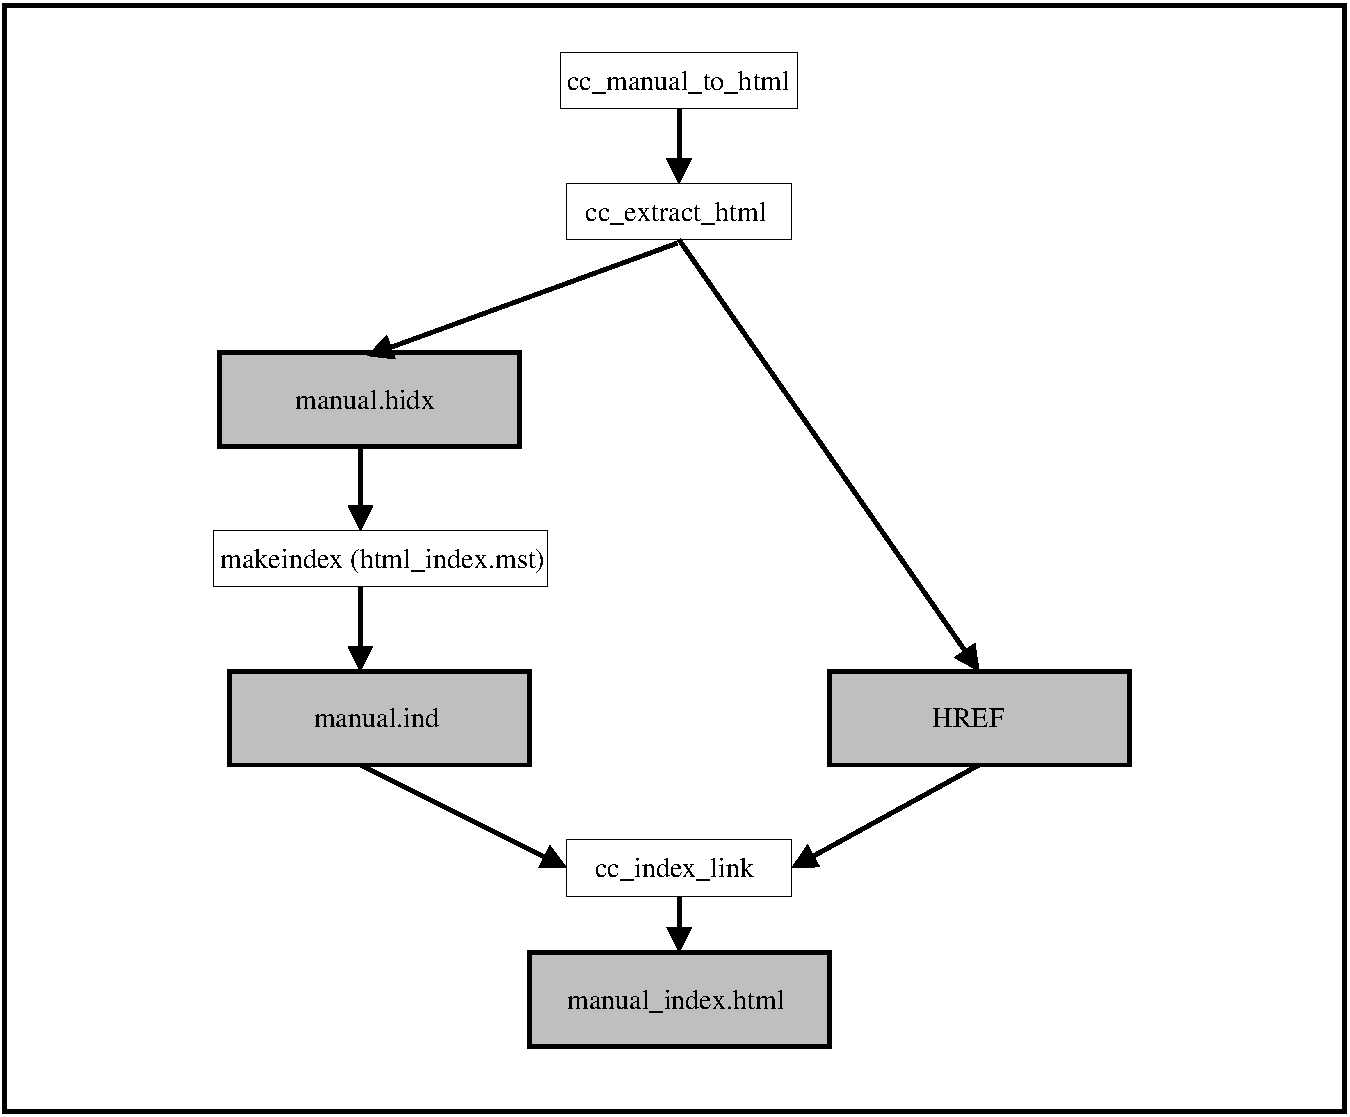
\includegraphics[width=1.0\textwidth]{tools_index}%
    \caption{The files and tools involved in the 
      process of creating the HTML index.}}
%    \label{ToolsOverviewFig}\figuretopindent
\begin{ccHtmlOnly}
<CENTER>
  <IMG SRC="./tools_index.gif" ALT="Files and tools used in manual writing">
</CENTER>
\end{ccHtmlOnly}
\end{figure}



\normalsize Program \verb|cc_extract_html| produces files
\verb|manual.hidx| and HREF. When the program finds a function that
produces the index position, it creates a new command for the {\tt
  makeindex} program. This new command contains the new index position
and its number. The number differs from the previous one by 2, since
otherwise if these numbers were consecutive it possible that {\tt
  makeindex} would create the page range out of these numbers instead
of separate page numbers.

Also, the program adds to file HREF an address of a link to an
appropriate place with yhe same number as the index position in file
\verb|mannual.hidx|.  After the whole index has been sorted by {\tt
  makeindex} (using the style file \verb|html_index.mst|), a file
\verb|manual.ind| is output. In this file the numbers of the links
have to be combined (attached) with appropriate link from file HREF.
This is done using program \verb|cc_index_link|. If the programm
\verb|cc_manual_to_html| is used with option {\tt -extended}, then the
program combines several \verb|manual.ind| files in to one
\verb|manual.ind| file, and their corresponding \verb|HREF| files into
one \verb|HREF| file. While doing so File \verb|HREF_counter| contains
the information on what should be the next number used for numbering
the links.

Examples:

Index position in file \verb|manual.hidx|:
  \begin{verbatim}
  \indexentry{functionality@ ??? functionality}{1040}
  \end{verbatim}

Link to this position in file \verb|HREF| :
  \begin{verbatim}
  1040 HREF="main.html#Index_anchor_302"
  \end{verbatim}

Sorted position in file \verb|manual.ind|:
 \begin{verbatim}
 <TABLE  CELLPADDING=0 CELLSPACING=0> <TR><TD>  ??? functionality ??? 
   1040 </TD></TR> </TABLE>
 \end{verbatim}

Index position after program \verb|cc_index_link| is run:
 \begin{verbatim}
 <TABLE  CELLPADDING=0 CELLSPACING=0> <TR><TD> 
   <A HREF="main.html#Index_anchor_302">  functionality</A> </TD></TR> </TABLE>
 \end{verbatim}


If a position in the index has many links, the arrows lead to these links.




\end{document}
